%%----------------------------------------------------------------------------------------
%	PACKAGES AND THEMES
%----------------------------------------------------------------------------------------
\PassOptionsToPackage{table}{xcolor}
\documentclass[aspectratio=169,xcolor=dvipsnames,svgnames,x11names,fleqn]{beamer}
% \documentclass[aspectratio=169,xcolor=dvipsnames,fleqn]{beamer}

\usetheme{RedVelvet}

\usefonttheme[onlymath]{serif}
\newcommand{\showanswers}{yes}
\usepackage{pifont} % For checkmarks and crosses

\usepackage{setspace}
\usepackage{xspace}
\usepackage{amsmath}
\usepackage{amssymb}
\usepackage{amsfonts}
\usepackage{color}
\usepackage{physics}
% \usepackage{mathbb}
\usepackage{rahul_math}
\usepackage{bigints}

\usepackage[utf8]{inputenc}
\usepackage[ruled,vlined]{algorithm2e}
\usepackage{amsmath}
\usepackage{amsfonts}

\usepackage{graphicx} % Allows including images
\usepackage{booktabs} % Allows the use of \toprule, \midrule and \bottomrule in tables
\usepackage{tikz,pgfplots}
\usepackage{mathtools}
\usepackage{subfigure}
\usetikzlibrary{arrows}
\usepackage{minted}
\definecolor{LightGray}{gray}{0.9}
\definecolor{cream}{rgb}{0.92, 0.9, 0.55}
\definecolor{lightblue}{rgb}{0.68, 0.85, 0.9}


\usepackage{xcolor-material}
\usetikzlibrary{fit}
\usetikzlibrary{matrix}
\tikzset{%
apple/.pic={
    \fill [MaterialBrown] (-1/8,0)  arc (180:120:1 and 3/2) coordinate [pos=3/5] (@)-- ++(1/6,-1/7)  arc (120:180:5/4 and 3/2) -- cycle;
    \fill [MaterialLightGreen500] (0,-9/10)  .. controls ++(180:1/8) and ++(  0:1/4) .. (-1/3,  -1) .. controls ++(180:1/3) and ++(270:1/2) .. (  -1,   0) .. controls ++( 90:1/3) and ++(180:1/3) .. (-1/2, 3/4) .. controls ++(  0:1/8) and ++(135:1/8) .. (   0, 4/7)
    }
    }

\newcommand{\leftdoublequote}{\textcolor{blue}{\scalebox{3}{``}}}

\newcommand{\rightdoublequote}{\textcolor{blue}{\scalebox{3}{''}}}


\usepackage{textcomp}
\usepackage{fontawesome}
\usepackage{tikz,pgfplots}
\usetikzlibrary{shapes.callouts}
\usetikzlibrary{arrows}
\usetikzlibrary{shapes.geometric, positioning}
\usetikzlibrary{matrix,positioning,decorations.pathreplacing,calc}
\usepackage{tikz-dependency}

\pgfplotsset{compat=1.8} % or newest version

\usetikzlibrary{positioning}


\usepackage{bm}
\usepackage{relsize}

\tcbuselibrary{skins, hooks}

\tikzset{basic/.style={draw,fill=MediumBlue!20,text width=1em,text badly centered}}
\tikzset{input/.style={basic,circle}}
\tikzset{weights/.style={basic,rectangle}}
\tikzset{functions/.style={basic,circle,fill=MediumBlue!10}}



\usepackage{listofitems} % for \readlist to create arrays
\tikzstyle{mynode}=[thick,draw=MediumBlue,fill=MediumBlue!20,circle,minimum size=22]


\usepackage{overpic}

%----------------------------------------------------------------------------------------
%	TITLE PAGE
%----------------------------------------------------------------------------------------

\usepackage{tikz-qtree,tikz-qtree-compat}
\usetikzlibrary{tikzmark}
\usetikzlibrary{calc}

\usetikzlibrary{fit}
\tikzset{%
apple/.pic={
    \fill [MaterialBrown] (-1/8,0)  arc (180:120:1 and 3/2) coordinate [pos=3/5] (@)-- ++(1/6,-1/7)  arc (120:180:5/4 and 3/2) -- cycle;
    \fill [MaterialLightGreen500] (0,-9/10)  .. controls ++(180:1/8) and ++(  0:1/4) .. (-1/3,  -1) .. controls ++(180:1/3) and ++(270:1/2) .. (  -1,   0) .. controls ++( 90:1/3) and ++(180:1/3) .. (-1/2, 3/4) .. controls ++(  0:1/8) and ++(135:1/8) .. (   0, 4/7)
}
}
\usepackage{tikz-qtree,tikz-qtree-compat}
\usetikzlibrary{tikzmark}
\usetikzlibrary{calc}

\usetikzlibrary{positioning}
\newcommand{\vect}[1]{\mathbf{#1}}
% Define styles
\tikzset{
    box/.style={
        rectangle,
        draw=black,
        fill=blue!20,
        text width=2.2cm,
        text centered,
        minimum height=0.8cm,
        font=\small
    },
    arrow/.style={
        ->,
        >=Stealth,
        line width=1.5pt,
        draw=black
    }
}


\usepackage{bm}
\usepackage{relsize}



\tikzset{basic/.style={draw,fill=MediumBlue!20,text width=1em,text badly centered}}
\tikzset{input/.style={basic,circle}}
\tikzset{weights/.style={basic,rectangle}}
\tikzset{functions/.style={basic,circle,fill=MediumBlue!10}}
\usetikzlibrary{arrows.meta, bending}
\usetikzlibrary{shapes.geometric, arrows.meta, positioning, fit, backgrounds}

\usepackage{listofitems} % for \readlist to create arrays
\tikzstyle{mynode}=[thick,draw=MediumBlue,fill=MediumBlue!20,circle,minimum size=22]


\newmdenv[
backgroundcolor=androidYellowLight,
linecolor=androidYellow,
linewidth=0.5pt,
roundcorner=10pt,
skipabove=\baselineskip,
skipbelow=\baselineskip
]{MintedFrame}

% Set minted options
\setminted{
fontsize=\footnotesize,
breaklines=true,
autogobble,
linenos,
frame=none
}


\title[CPE 487/587: Deep Learning]{CPE 486/586: Deep Learning for Engineering Applications} % The short title appears at the bottom of every slide, the full title is only on the title page
\subtitle{08 Diffusion Models}

\author[Rahul Bhadani] {{\Large \textbf{Rahul Bhadani}}}

\institute[UAH] % Your institution as it will appear on the bottom of every slide, maybe shorthand to save space
{
    Electrical \& Computer Engineering,  The University of Alabama in Huntsville
}
\date

% \titlegraphic{
%    \includegraphics[width=0.4\linewidth]{figures/UAH_primary.png}
% }

\begin{document}

%-------------------------------------------------
\begin{frame}
    \titlepage
\end{frame}

%-------------------------------------------------
\begin{frame}{Outline}
    \backgroundtableofcontents
\end{frame}

%------------------------------------------------
\begin{frame}{}
    \begin{center}
        \huge \bf \color{DarkBlue}
        Motivation 
    \end{center}
    \end{frame}
    
\begin{frame}{Generative Models}

\resizebox{0.7\textwidth}{!}
{
\begin{tikzpicture}[
    font=\sffamily\small,
    >=Stealth,
    node distance=1.0cm and 1.0cm,
    box/.style={rectangle, draw=Blue, fill=BlueLight, minimum width=0.6cm, minimum height=2cm, thick},
    input/.style={box, draw=Sage, fill=SageLight},
    latent/.style={rectangle, draw=Rust, fill=RustPale, minimum size=0.6cm, thick},
    trapezoid/.style={trapezium, draw=Sage, fill=SageLight, shape border rotate=270, minimum height=1.5cm, trapezium stretches body, thick},
    trapezoid_inv/.style={trapezoid, draw=Blue, fill=BlueLight, shape border rotate=90},
    label_node/.style={align=left, font=\sffamily\bfseries, text width=8cm}
]

% --- GAN ---
\node[label_node] (gan_lab) {GAN: \textnormal{Adversarial training}};
\node[box, right=of gan_lab] (gan_x_prime_in) {$\mathbf{x}'$};
\node[input, right=0.2cm of gan_x_prime_in] (gan_x) {$\mathbf{x}$};
\node[trapezoid, right=of gan_x] (disc) {\begin{tabular}{c} Discriminator \\ $D(\mathbf{x})$ \end{tabular}};
\node[circle, draw=Ink, fill=BlueLight!50!SageLight, right=0.4cm of disc, thick] (prob) {0/1};
\node[latent, right=0.6cm of prob] (gan_z) {$\mathbf{z}$};
\node[trapezoid_inv, right=of gan_z] (gen) {\begin{tabular}{c} Generator \\ $G(\mathbf{z})$ \end{tabular}};
\node[box, right=of gen] (gan_x_prime_out) {$\mathbf{x}'$};

\draw[->] (gan_x) -- (disc);
\draw[->] (disc) -- (prob);
\draw[->] (gan_z) -- (gen);
\draw[->] (gen) -- (gan_x_prime_out);

% --- VAE ---
\node[label_node, below=4cm of gan_lab] (vae_lab) {VAE: \textnormal{maximize variational lower bound}};
\node[input, right=1.6cm of vae_lab] (vae_x) {$\mathbf{x}$};
\node[trapezoid, right=of vae_x] (enc) {\begin{tabular}{c} Encoder \\ $q_\wbf(\mathbf{z}|\mathbf{x})$ \end{tabular}};
\node[latent, right=of enc] (vae_z) {$\mathbf{z}$};
\node[trapezoid_inv, right=of vae_z] (dec) {\begin{tabular}{c} Decoder \\ $p_\vbf(\mathbf{x}|\mathbf{z})$ \end{tabular}};
\node[box, right=of dec] (vae_x_prime) {$\mathbf{x}'$};

\draw[->] (vae_x) -- (enc);
\draw[->] (enc) -- (vae_z);
\draw[->] (vae_z) -- (dec);
\draw[->] (dec) -- (vae_x_prime);

% --- Flow ---
\node[label_node, below=3cm of vae_lab] (flow_lab) {Flow-based models: \textnormal{Invertible transform of distributions}};
\node[input, right=1.6cm of flow_lab] (flow_x) {$\mathbf{x}$};
\node[rectangle, draw=Sage, fill=SageLight, minimum width=1.5cm, minimum height=1.5cm, thick, right=of flow_x] (flow_f) {\begin{tabular}{c} Flow \\ $f(\mathbf{x})$ \end{tabular}};
\node[latent, right=of flow_f] (flow_z) {$\mathbf{z}$};
\node[rectangle, draw=Blue, fill=BlueLight, minimum width=1.5cm, minimum height=1.5cm, thick, right=of flow_z] (flow_inv) {\begin{tabular}{c} Inverse \\ $f^{-1}(\mathbf{z})$ \end{tabular}};
\node[box, right=of flow_inv] (flow_x_prime) {$\mathbf{x}'$};

\draw[->] (flow_x) -- (flow_f);
\draw[->] (flow_f) -- (flow_z);
\draw[->] (flow_z) -- (flow_inv);
\draw[->] (flow_inv) -- (flow_x_prime);

% --- Diffusion ---
\node[label_node, below=3cm of flow_lab] (diff_lab) {Diffusion models: \textnormal{Gradually add Gaussian noise and then reverse}};
\node[input, right=1.6cm of diff_lab] (x0) {$\mathbf{x}_0$};
\node[rectangle, draw=Gold, fill=GoldLight!40, minimum width=0.6cm, minimum height=2cm, thick, right=0.6cm of x0] (x1) {$\mathbf{x}_1$};
\node[rectangle, draw=Gold, fill=GoldLight!70, minimum width=0.6cm, minimum height=2cm, thick, right=0.6cm of x1] (x2) {$\mathbf{x}_2$};
\node[right=0.8cm of x2] (dots) {$\dots \dots$};
\node[rectangle, draw=Rust, fill=RustPale, minimum width=0.6cm, minimum height=2cm, thick, right=0.8cm of dots] (diff_z) {$\mathbf{z}$};

\draw[->] ([yshift=2mm]x0.east) -- ([yshift=2mm]x1.west);
\draw[->, dashed] ([yshift=-2mm]x1.west) -- ([yshift=-2mm]x0.east);
\draw[->] ([yshift=2mm]x1.east) -- ([yshift=2mm]x2.west);
\draw[->, dashed] ([yshift=-2mm]x2.west) -- ([yshift=-2mm]x1.east);
\draw[->] ([yshift=2mm]x2.east) -- ([yshift=2mm]dots.west);
\draw[->, dashed] ([yshift=-2mm]dots.west) -- ([yshift=-2mm]x2.east);
\draw[->] ([yshift=2mm]dots.east) -- ([yshift=2mm]diff_z.west);
\draw[->, dashed] ([yshift=-2mm]diff_z.west) -- ([yshift=-2mm]dots.east);

\end{tikzpicture}
}

\end{frame}

\begin{frame}{Why Diffusion Model and not VAE}

\begin{itemize}
\item VAE operates on a single-step compression - expansion idea.
\item High-frequency details like textures, sharp texts, etc are discarded in attempt to minimize the loss.
\end{itemize}

\vspace{15pt}
\begin{center}
Diffusion Models attempt to solve this by breaking down each step into multiple tiny steps.
\end{center}

\end{frame}
    
    \begin{frame}{Diffusion Model as the State of the Art for Generative Models}
    \begin{center}
               \includegraphics[width=0.22\textwidth, trim={0 0 0 0}, clip]{figures/Midjourney_2.png}
              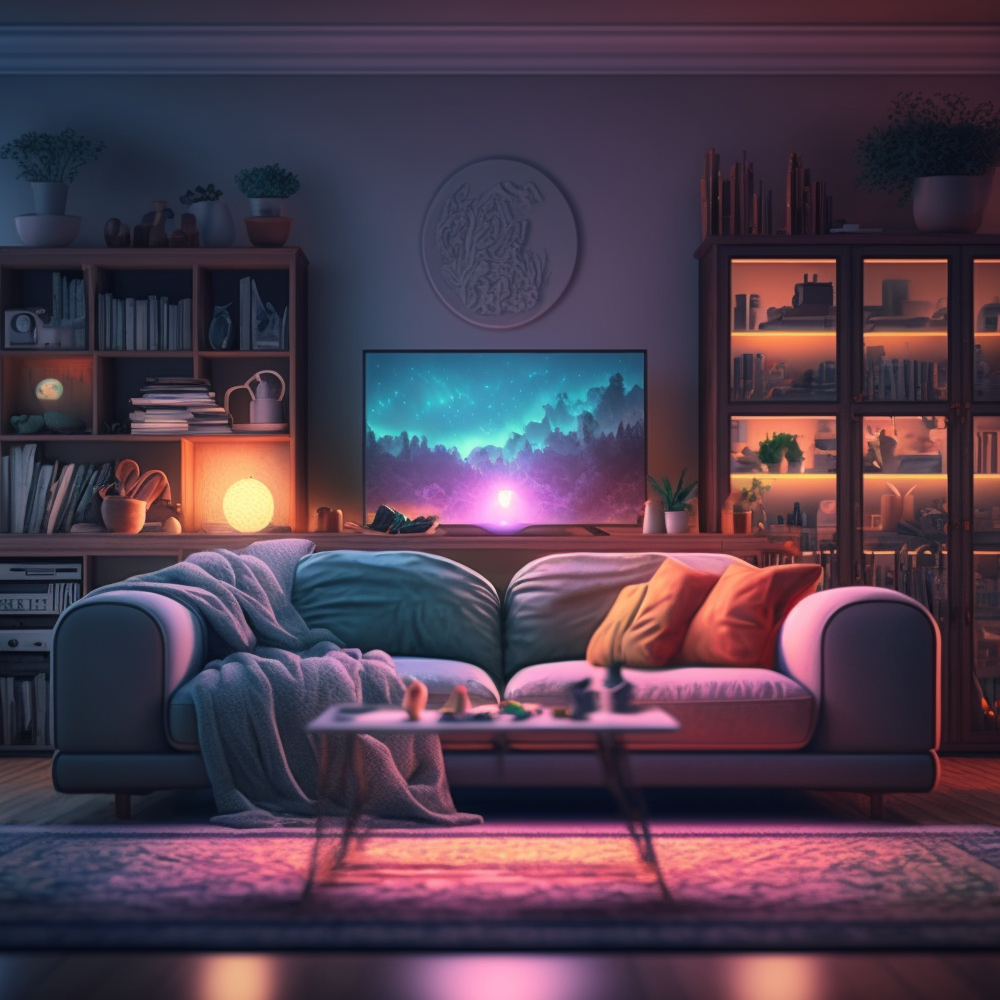
\includegraphics[width=0.22\textwidth, trim={0 0 0 0}, clip]{figures/Midjourney_1.png}
             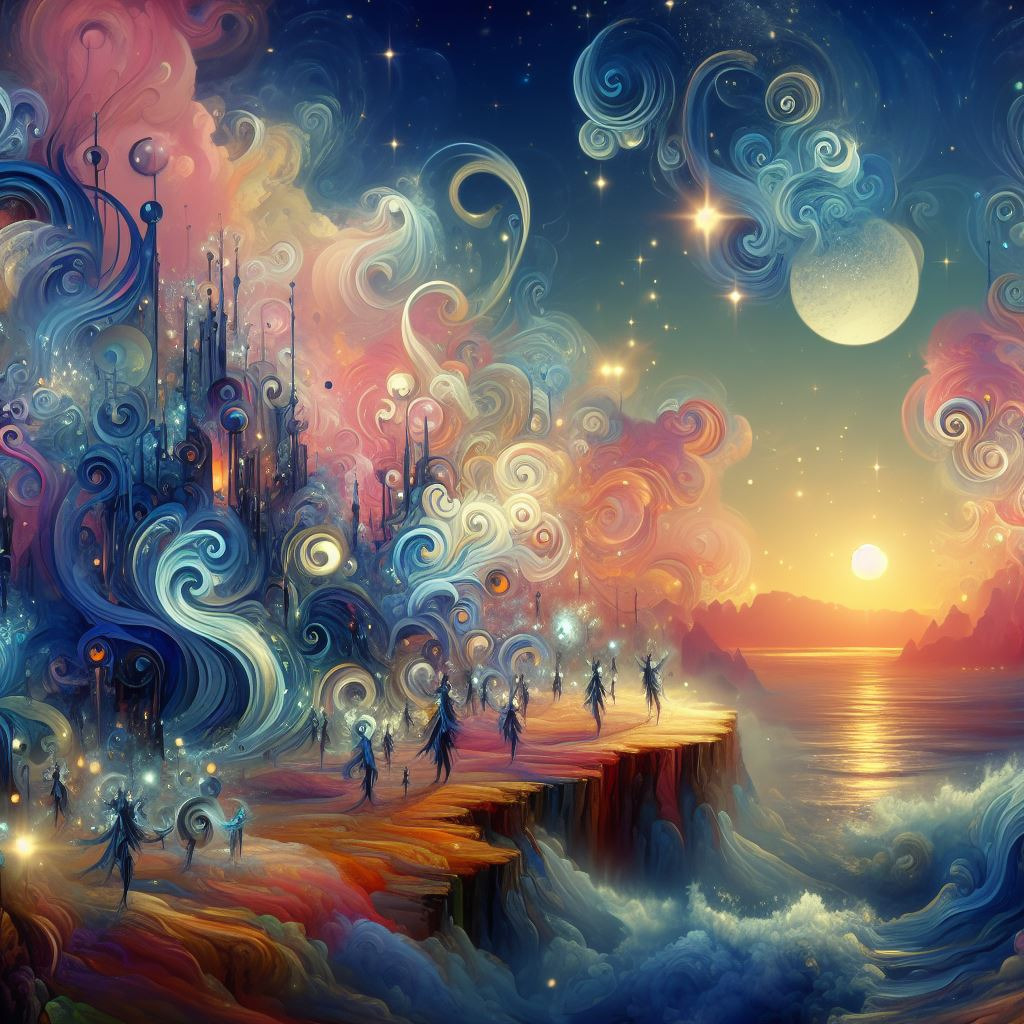
\includegraphics[width=0.22\textwidth, trim={0 0 0 0}, clip]{figures/pilot_1.png}
             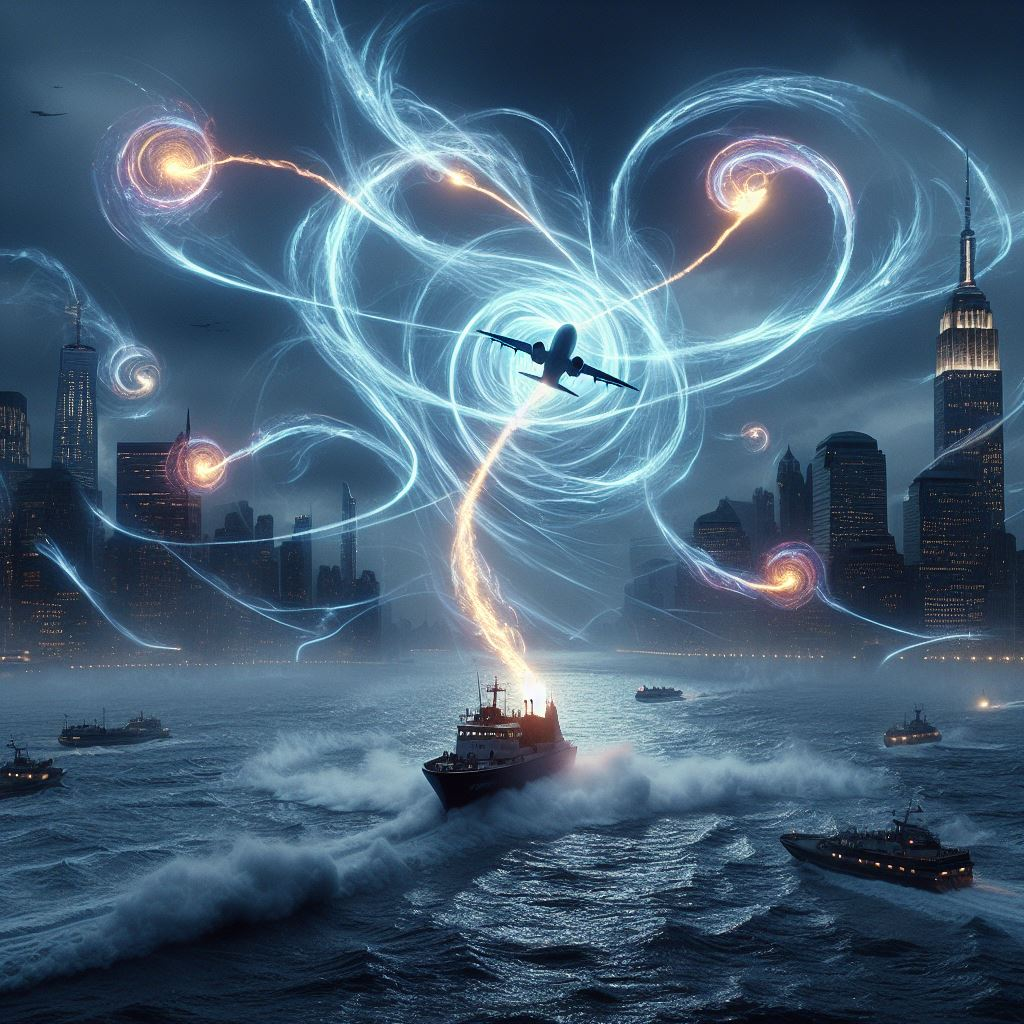
\includegraphics[width=0.22\textwidth, trim={0 0 0 0}, clip]{figures/pilot_2.png}
             
                \textbf{Figures created using Midjourney v4 and GPT-4.}
    \end{center}
      
       
    \end{frame}
    
    \begin{frame}{Diffusion Model are non-Adversarial}
    \begin{center}
    \textbf{Adversarial Models such as GAN are difficult to train.}
    
      
\includegraphics[width=0.19\textwidth, trim={0 0 0 0}, clip]{figures/hundred.png}
    
    \textbf{Discriminator can be too good!!}
    \end{center}
        
    \end{frame}
    

    %------------------------------------------------
    \section{Diffusion Models}
    %------------------------------------------------
    
    %------------------------------------------------
    \begin{frame}{}
    \begin{center}
        \huge \bf \color{DarkBlue}
        Diffusion Models 
    \end{center}
    \end{frame}
    
    
    %------------------------------------------------
    \begin{frame}{Inspiration behind Diffusion Model}
    \begin{center}
    {
    \Large \bf \color{DarkViolet}
        Inspired by non-equilibrium behavior in Thermodynamics
    }
    
     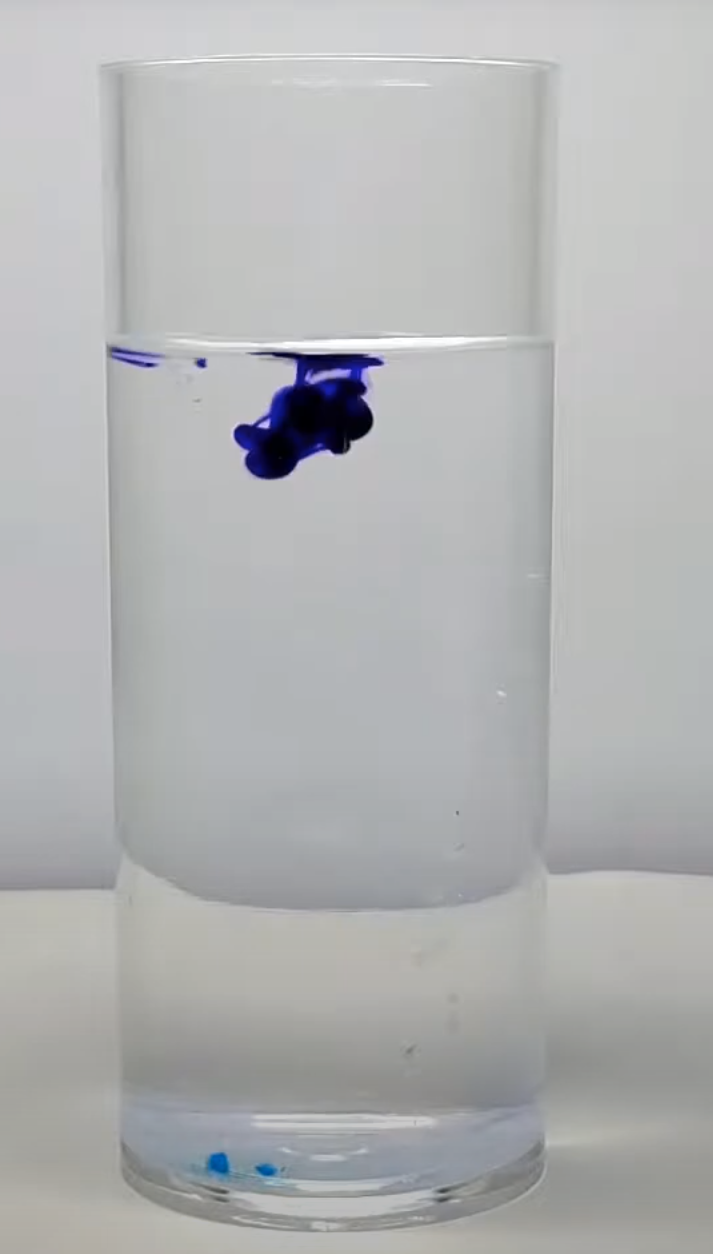
\includegraphics[width=0.19\textwidth, trim={0 0 0 0}, clip]{figures/inkdrop_start.png}
     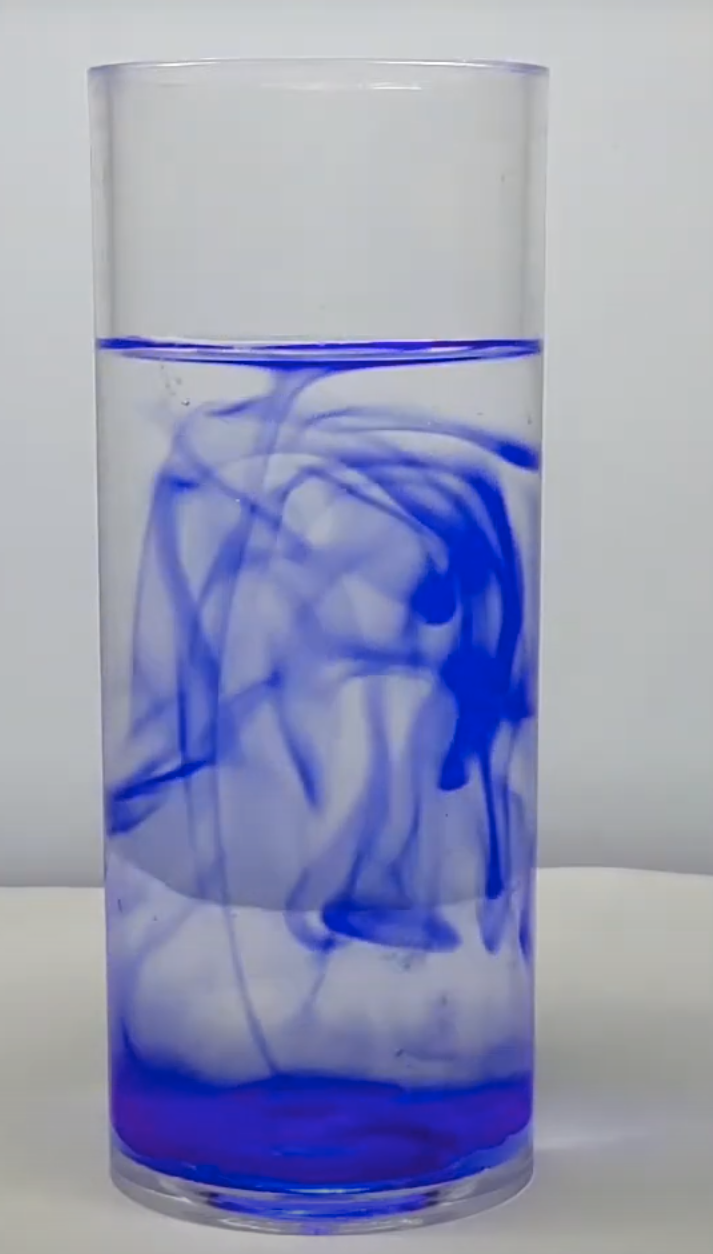
\includegraphics[width=0.19\textwidth, trim={0 0 0 0}, clip]{figures/inkdrop_later.png}
    
    {
    \Large \bf \color{Magenta}
        The drop of ink eventually diffuses into the water until it reaches equilibrium.
    }
    \end{center}
    \end{frame}
    
    %------------------------------------------------
    \begin{frame}{Intuition behind Diffusion Model}
    \begin{center}
    {
    \large \bf \color{DarkViolet}
        In the physical world, the reversal of the diffusion process is not possible. But that's what the diffusion model is trying to do.
    }
    
    \vspace{20pt}
    \begin{columns}
    \column{0.44\linewidth}
    \raggedleft
     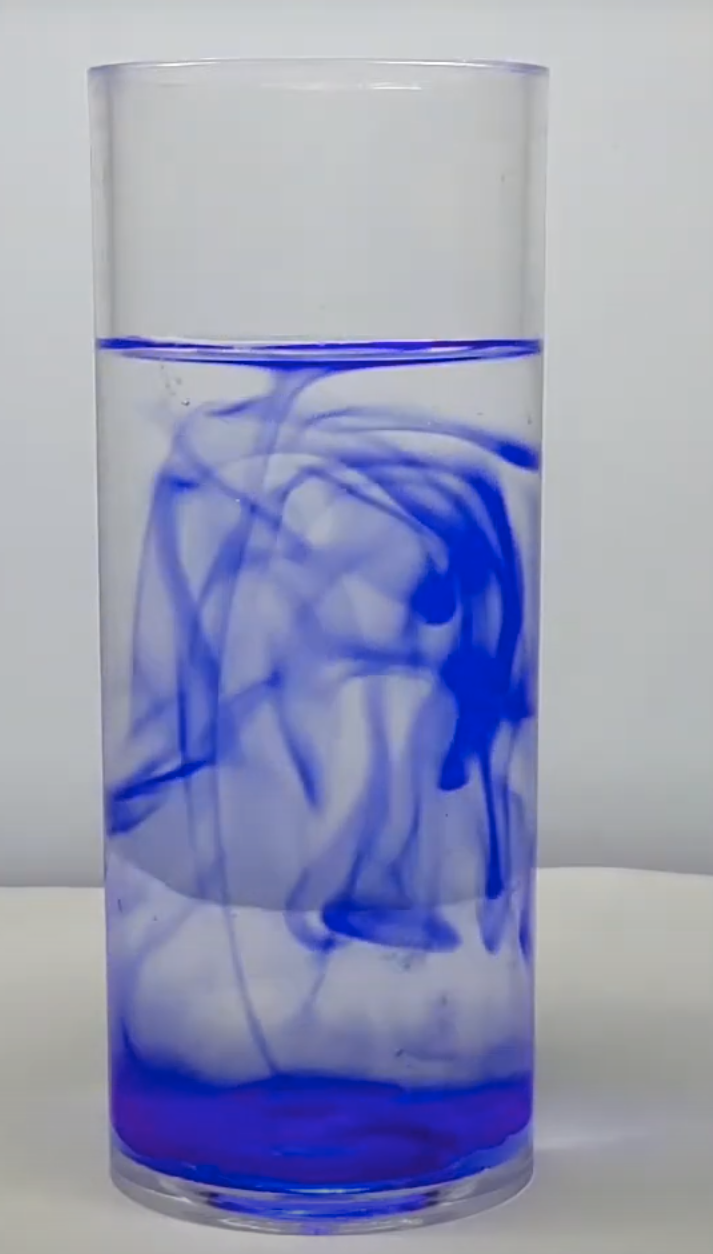
\includegraphics[width=0.44\textwidth, trim={0 0 0 0}, clip]{figures/inkdrop_later.png}
     \column{0.12\linewidth}
     \raggedleft
    \Huge \faArrowCircleRight~~
     \column{0.44\linewidth}
     \raggedright
     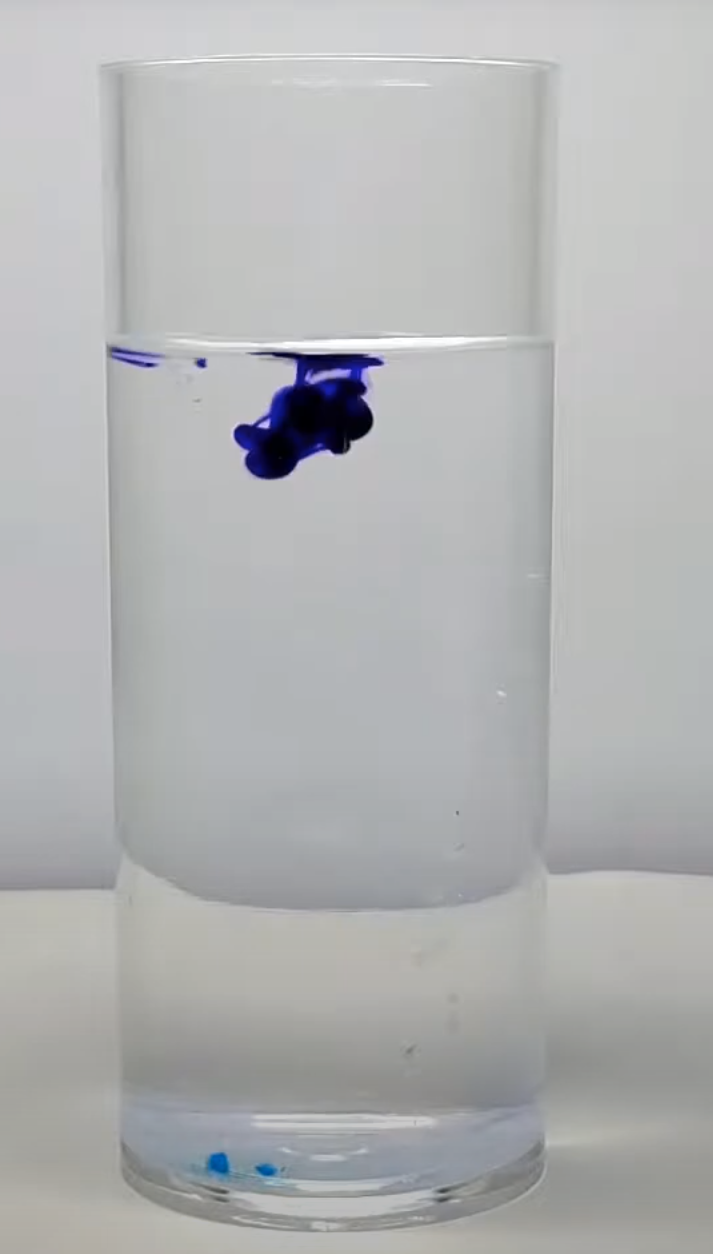
\includegraphics[width=0.44\textwidth, trim={0 0 0 0}, clip]{figures/inkdrop_start.png}
    \end{columns} 
    \end{center}
    \end{frame}
    
    %------------------------------------------------
    \begin{frame}{Intuition behind Diffusion Model}
    \begin{center}
    \Large \bf \color{WildStrawberry}
        In the ink-water diffusion example, the drop of the ink at one spot includes some information.
    \end{center}
    \vspace{20pt}
    \begin{center}
    \Large \bf \color{JungleGreen}
      As the diffusion process progresses, we lose information, and eventually, we only have noise.
    \end{center}
    \end{frame}
    
    
    %------------------------------------------------
    \begin{frame}{Intuition behind Diffusion Model}
    \begin{center}
    {\Large \bf \color{WildStrawberry}
      In the image domain:
    }
    \vspace{15pt}
      \begin{columns}
          \column{0.3\linewidth}
               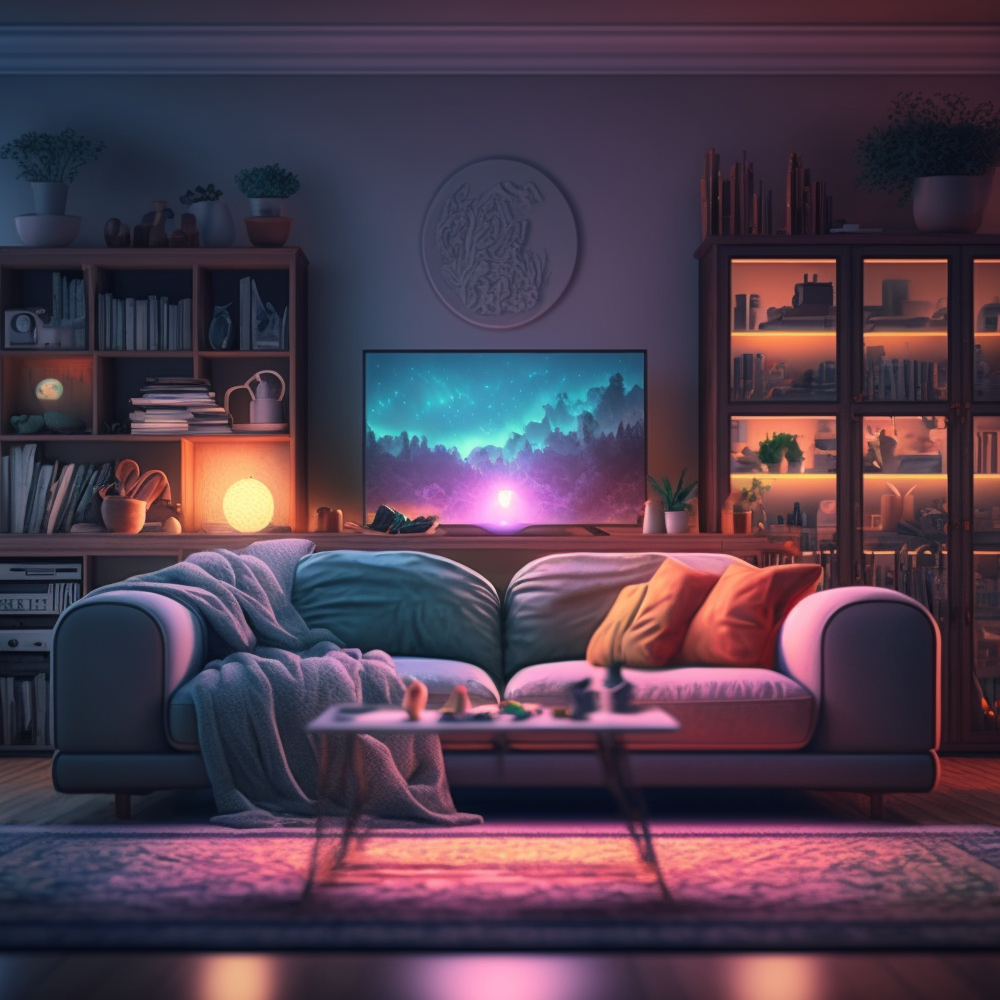
\includegraphics[width=0.82\textwidth, trim={0 0 0 0}, clip]{figures/Midjourney_1.png}
               Clear information
    \column{0.3\linewidth}
               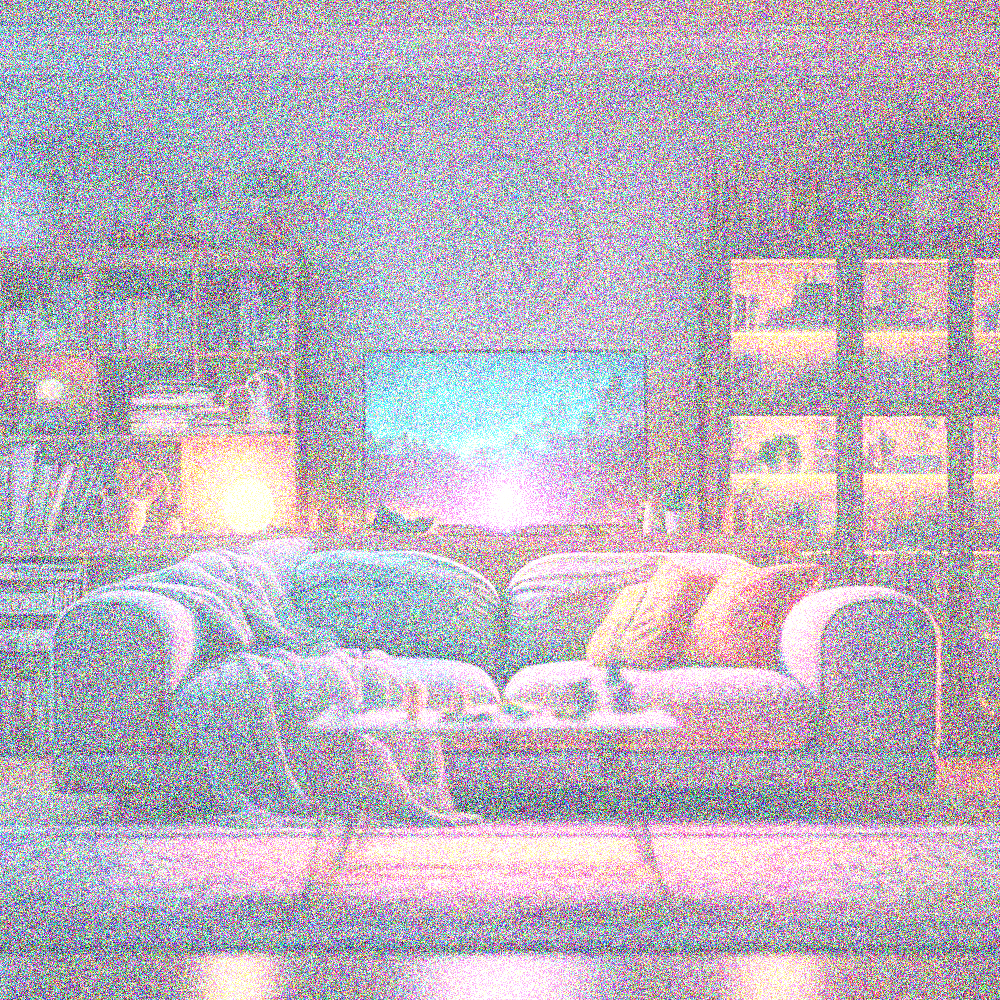
\includegraphics[width=0.82\textwidth, trim={0 0 0 0}, clip]{figures/Midjourney_1_noisy_mid.png}
               Some loss of information
               \column{0.3\linewidth}
               
\includegraphics[width=0.82\textwidth, trim={0 0 0 0}, clip]{figures/Midjourney_1_noisy.png}
               Just noise
      \end{columns}
      \vspace{15pt}
      {\Large \bf \color{NavyBlue}
      Working backward from just noise to a proper image is what a diffusion model tries to achieve.
    }
    \end{center}
    \end{frame}
    
    %------------------------------------------------
    \begin{frame}{The Working Principle of the Diffusion Model}
    \begin{center}
      {\Large \bf \color{purple}
        Add noise to the original image and then later learn how to reverse this noise process.
    }
    \end{center}
    \end{frame}
    
    %------------------------------------------------
    \begin{frame}{The Working Principle of the Diffusion Model}
    \begin{center}
      {\Large \bf \color{purple}
        Apply noise following a Markov chain/Markov Process.
    }
    \vspace{15pt}
      \begin{columns}
          \column{0.21\linewidth}
               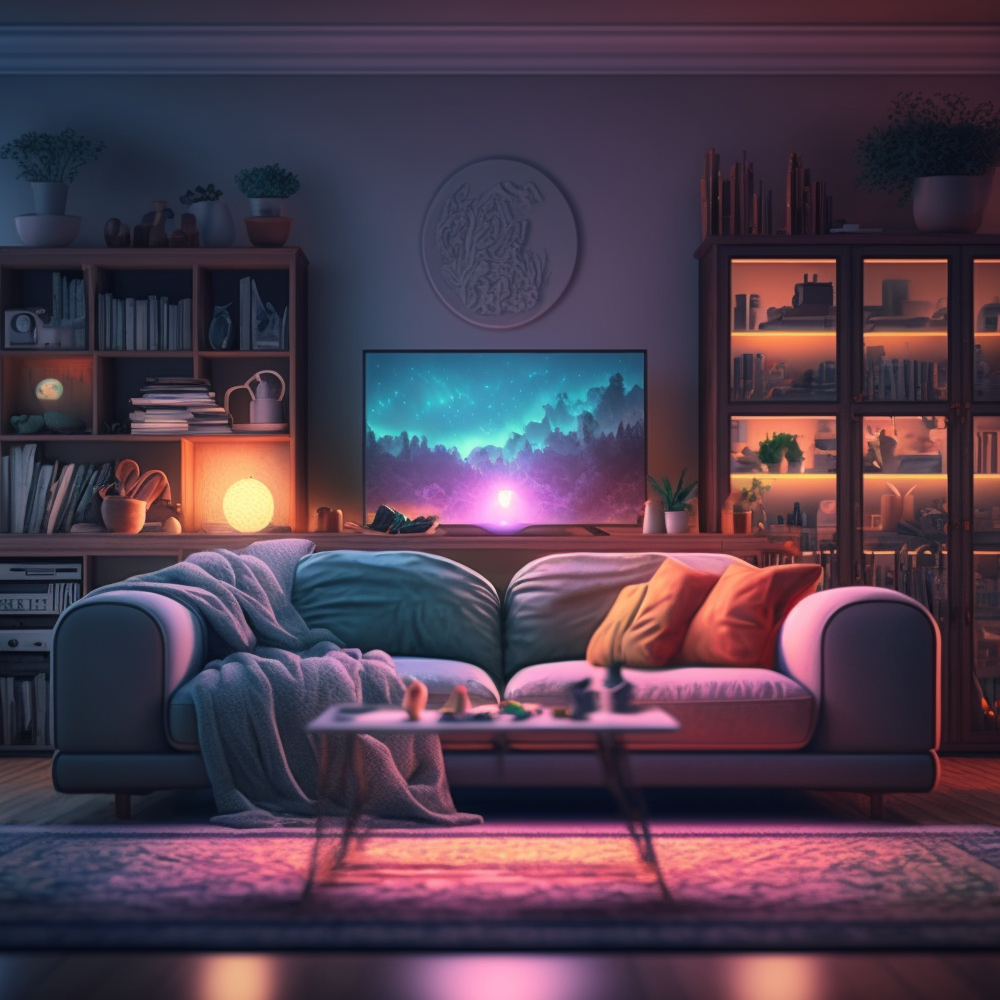
\includegraphics[width=0.82\textwidth, trim={0 0 0 0}, clip]{figures/Midjourney_1.png}
               \column{0.05\linewidth}
               \huge \faArrowCircleRight
               \column{0.21\linewidth}
               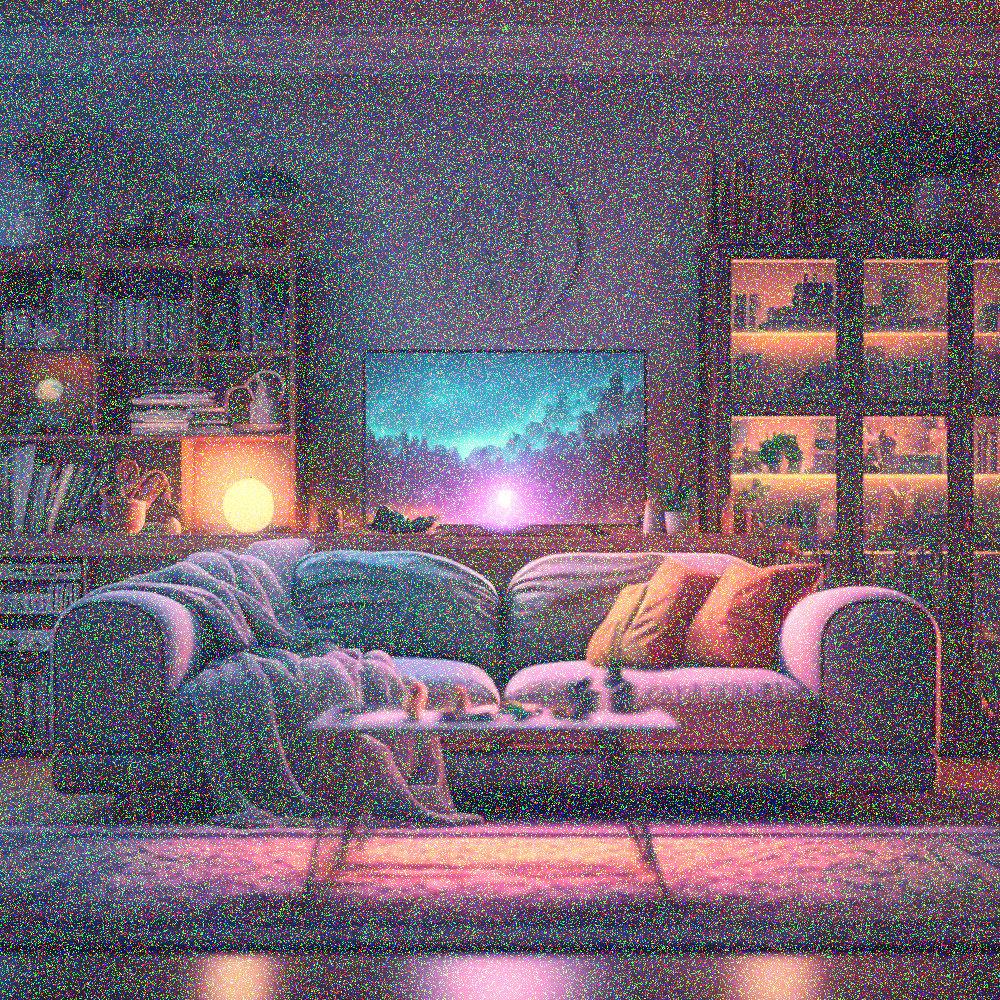
\includegraphics[width=0.82\textwidth, trim={0 0 0 0}, clip]{figures/Midjourney_1_noisy_early.png}
                \column{0.05\linewidth}
               \huge \faArrowCircleRight
            \column{0.21\linewidth}
               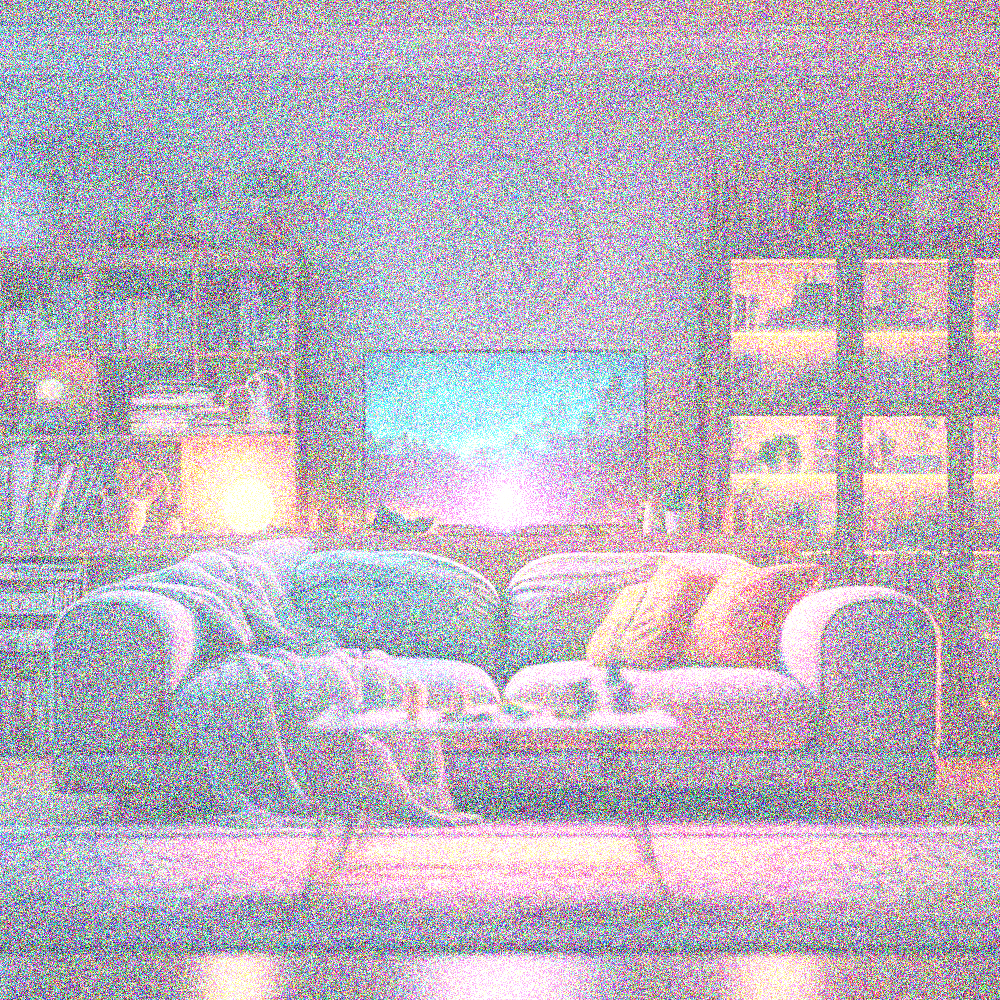
\includegraphics[width=0.82\textwidth, trim={0 0 0 0}, clip]{figures/Midjourney_1_noisy_mid.png}
                \column{0.05\linewidth}
               \huge \faArrowCircleRight
               \column{0.21\linewidth}
               
\includegraphics[width=0.82\textwidth, trim={0 0 0 0}, clip]{figures/Midjourney_1_noisy.png}
      \end{columns}
      \vspace{15pt}
        {\large \bf \color{MediumBlue}
       At each time step, we add a little bit of noise to the image until the image only consists of the noise. We have 100-1000 long Markov chain.
    }
    \end{center}
    \end{frame}
    
    \begin{frame}{Noise in the Diffusion Model}
        \begin{center}
        {\large \bf \color{MediumBlue}
            Gaussian Noise: $\Ncal(\mu , \sigma^2)$
        }
         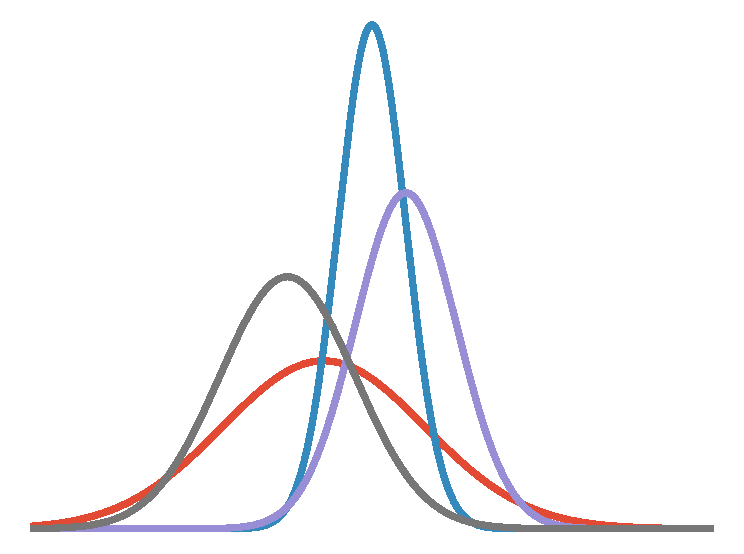
\includegraphics[width=0.32\textwidth, trim={0 0 0 0}, clip]{figures/gaussian_distribution.pdf}
    
          \begin{tabular}{|c|}
    \hline
    25 \\
    \hline
    67 \\
    \hline
    \end{tabular} + $\Ncal(\mu , \sigma^2)$  =     \begin{tabular}{|c|}
    \hline
    26.63 \\
    \hline
    66.55 \\
    \hline
    \end{tabular} 
    
      \vspace{15pt}
    Repeat the process.
        \end{center}
    \end{frame}
    
    \begin{frame}{Idea Behind Removing the Noise (Working Backward)}
        \begin{center}
               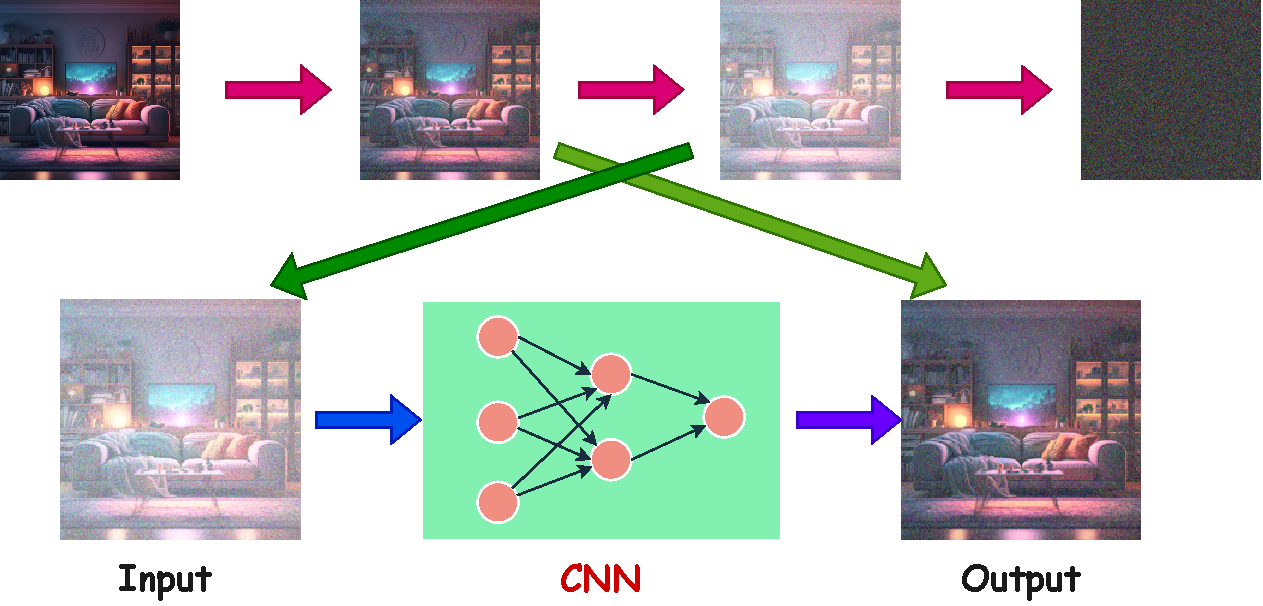
\includegraphics[width=0.75\textwidth, trim={0 0 0 0}, clip]{figures/DiffusionModel.pdf}
    
               \vspace{15pt}
                {\large \bf \color{MediumGreen}
       The type of CNN used in the original paper is called UNet. (Transformer can also be used). In general, we call them \textit{\underline{backbone}} models.
    }
        \end{center}
    \end{frame}
    
    \begin{frame}{UNet Architecture}
        \begin{center}
               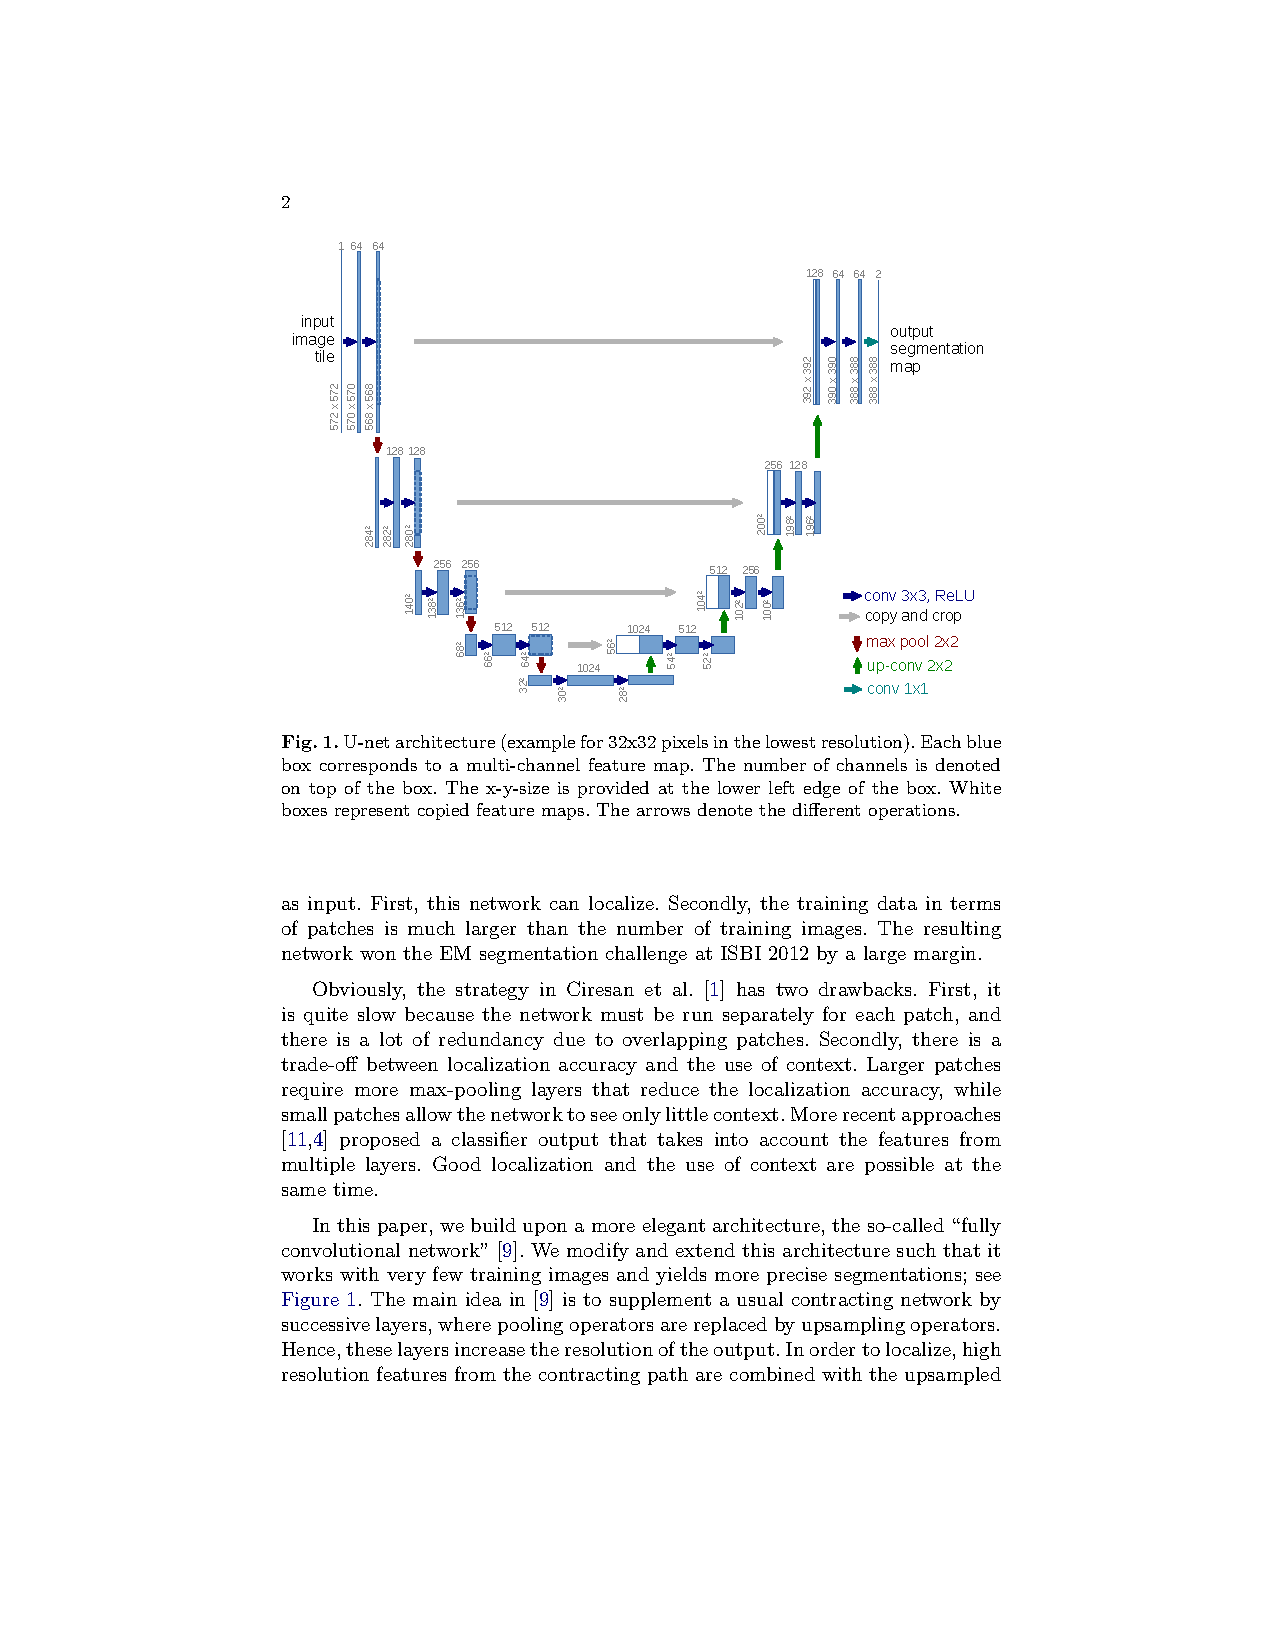
\includegraphics[width=0.67\textwidth, trim={100 450 120 100}, clip]{figures/UNet.pdf}
    
               \vspace{15pt}
                {\large \bf \color{MediumRed}
    Source: \url{https://arxiv.org/pdf/1505.04597.pdf}
    }
        \end{center}
    \end{frame}
    
    \begin{frame}{UNet Architecture for Diffusion}
    \begin{itemize}
        \item U-net consists of a series of up/down sampling convolution blocks which are connected via residual connection, along with a middle block. This set up allow allows one to global location and context at the same time in the learning process. It works with very few training samples and provides better performance for segmentation tasks.
    
        \item  In the Diffusion model, UNet architecture is combined with time-step embedding called sinusoidal embedding. This is similar to the positional embedding seen in the transformer. This block combines sinusoidal embedding and convolution layers to learn the time step of the noisy images in the diffusion process.
    \end{itemize}
       
    \end{frame}
    
    \begin{frame}{Historical Timeline}
\small
\resizebox{1.2\textheight}{!}
{
\begin{tikzpicture}
\draw[Gold!40,line width=1pt] (0,0) -- (0,-7.8);
\foreach \y/\yr/\title/\desc in {
  0.0/2015/{Sohl-Dickstein et al.}/{Thermodynamic diffusion framework. Largely overlooked.},
  -1.1/2019/{Song \& Ermon}/{Score-based models with Langevin dynamics -- a parallel track.},
  -2.2/2020/{Ho et al.\ (DDPM)}/{Simplified $\varepsilon$-prediction; quality rivals GANs. The field ignites.},
  -3.3/2021/{SDEs + DDIM}/{Song et al.\ unify via SDEs. DDIM gives $10$--$50\times$ speedup.},
  -4.4/2022/{Stable Diffusion}/{Rombach et al.: latent diffusion; open-source text-to-image.},
  -5.5/2023/{DiT + Flow Matching}/{Transformers replace U-Nets. Consistency models (1-step).},
  -6.6/2024+/{FLUX, SD3, Sora}/{Frontier image, video, science models at production scale.}
}{
  \filldraw[Gold] (0,\y) circle (3.5pt);
  \node[font=\tiny\ttfamily\bfseries,text=Gold,right=0.0cm,
        minimum width=1.2cm,align=right] at (-2.2,\y) {\yr};
  \node[font=\scriptsize\bfseries,text=Ink,right=0.35cm] at (0,{\y+0.15}) {\title};
  \node[font=\scriptsize,text=InkLight,right=0.35cm,text width=10.5cm]
    at (0,{\y-0.22}) {\desc};
}
\end{tikzpicture}
}
\end{frame}

    %------------------------------------------------
    \section{Mathematical Framework for Diffusion Models}
    %------------------------------------------------
 
    
    
    %------------------------------------------------
    \begin{frame}{}
    \begin{center}
        \huge \bf \color{DarkBlue}
        Mathematical Framework for Diffusion Models: Denoising Diffusion Probabilistic Model (DDPM)
    \end{center}
    \end{frame}
    
    \begin{frame}{Generated Samples from DDPM}
    
    \begin{columns}
    
    \column{0.48\linewidth}
    \begin{center}
    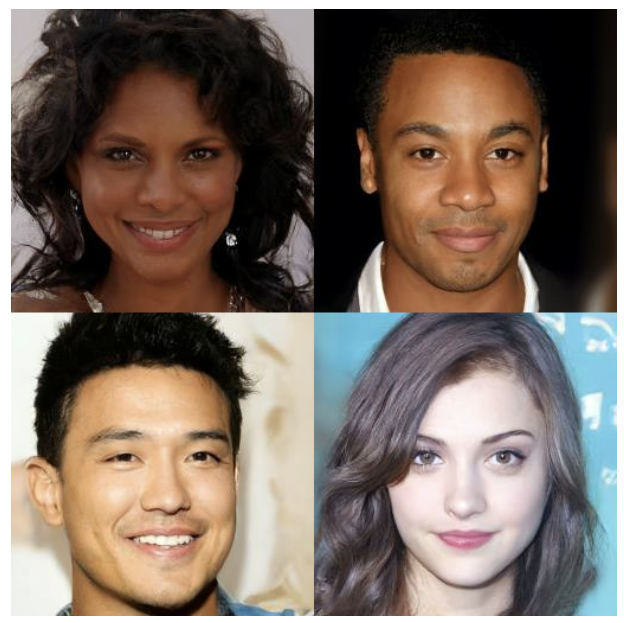
\includegraphics[width=0.68\linewidth]{figures/ddpm_samples.png}
    
    \footnotesize
    
    Source: Denoising Diffusion Probabilistic Models \url{https://proceedings.neurips.cc/paper/2020/file/4c5bcfec8584af0d967f1ab10179ca4b-Paper.pdf}
    \end{center}
    
    
    \column{0.5\linewidth}

\begin{tcolorbox}[vcHighlight, title={\color{vcDeep}\bfseries\small Definition }]
A diffusion probabilistic model (a \textbf{diffusion model} for brevity) is a parameterized Markov chain trained using variational inference to produce samples matching the data after finite time.

\vspace{10pt}

\tiny Ho, Jonathan, Ajay Jain, and Pieter Abbeel. "Denoising diffusion probabilistic models." Advances in neural information processing systems 33 (2020): 6840-6851.

\end{tcolorbox}

    
    
    \end{columns}
    \end{frame}
    
    \begin{frame}{Background Terminology}
    
    \begin{itemize}
    \item $\xbf_0 \sim q(\xbf_0)$: the original data.
    \item $\xbf_1, \xbf_2, \cdots, \xbf_T$: latent dimensions of the same dimensionality as $\xbf_0$.
    \item Joint distribution of the reverse process: $ p_\theta(\xbf_0, \xbf_1, \xbf_2, \cdots, \xbf_T)$ or  $p_\theta(\xbf_{0:T})$  in short.
    \item Reverse process is defined s Markov chain with a learned Gaussian transition start at $p(\xbf_T) = \Ncal(\xbf_T, \bm 0, \Ibf)$.
    \item Approximate posterior $q(\xbf_{1:T} | \xbf_0)$, called forward process or diffusion process in the realm of diffusion model.
    \item The approximate posteror is fixed to a Markov process (or Markov chain) that adds Gaussain noise little by little according to a variance schedule $\beta_1, \beta_2, \cdots, \beta_T$.
    \end{itemize}
    
    \end{frame}
    
    \begin{frame}{Formulating Diffusion Model: Forward Process}
        \begin{center}
        \begin{itemize}
            \item   Consider an original image data sampled from the real distribution $\xbf_0 \sim q(\xbf)$.
            \item We add small Gaussian noise to the sample data in $T$ steps, producing a sequence of noisy samples $\xbf_1, \xbf_2, \cdots, \xbf_T$.
            \item The step sizes are controlled by the diffusion rate  $\{\beta_t \in (0, 1)\}$, a hyperparameter.
            \item The data sample $\xbf_0$ slowly loses its distinguishable features as the step $t$ becomes larger. 
        \end{itemize}
        \end{center}
    \end{frame}
    
    \begin{frame}{Forward Process: Adding Noise}
        \begin{center}
              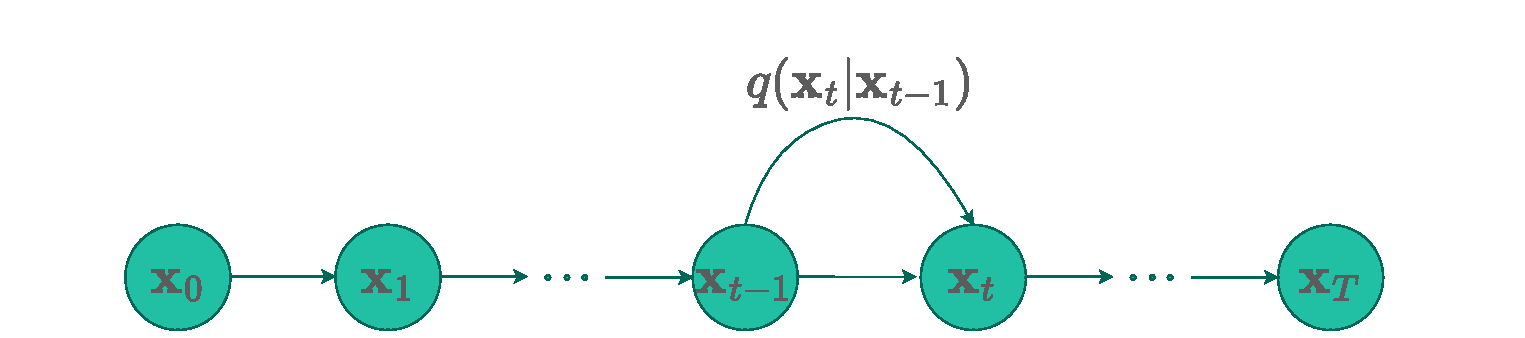
\includegraphics[width=0.99\textwidth, trim={0 0 0 0}, clip]{figures/Diffusion_Model_Forward_Process.pdf}
              
              \vspace{10pt}
    
              \begin{itemize}
                  \item If the noise to be added is Gaussian, then we use the analytical distribution (also known as \textbf{transition kernel}) of the noisy data at time step $t$ as $q(\xbf_t | \xbf_{t-1}) = \Ncal(\xbf_t; \sqrt{1-\beta_t}\xbf_{t-1}, \beta_t\Ibf)$. \textbf{Note: this is a design choice.}
                  \item The conditional distribution of the noisy data for the subsequent Markov chain (i.e. joint distribution of $\xbf_1, \xbf_2, \cdots, \xbf_T$) is written as $$q(\xbf_1, \xbf_2, \cdots, \xbf_T | \xbf_0) = q(\xbf_{1:T} | \xbf_0) = {\prod}_{t=0}^T q(\xbf_t|\xbf_{t-1})$$.
              \end{itemize}
        \end{center}
    \end{frame}
    
    \begin{frame}{Forward Process: Adding Noise}
    \begin{itemize}
        \item We sample $\xbf_t$ at any arbitrary time step $t$ in a closed form using reparameterization trick
    
        $$
        \alpha_1  = 1 - \beta_t, \quad \bar{\alpha}_t = \prod_{i=1}^t   \alpha_i.
        $$
        This can help us write analytical form of $q(\xbf_t | \xbf_0)$ for all $t \in \{0, 1, \cdots, T\}$ as
        $$
        q(\xbf_t | \xbf_0) = \Ncal(\xbf_t ; \sqrt{\bar{\alpha}_t}\xbf_0, (1-\bar{\alpha}_t)\Ibf).
        $$
        \item Given $\xbf_0$, we can sample $\xbf_t$, by supplying small Gaussian perturbation $\varepsilon \sim\Ncal(0, \Ibf)$ and applying a transformation
        $$
        \xbf_t = \sqrt{\bar{\alpha}_t}\xbf_0 + \sqrt{(1-\bar{\alpha}_t)}\varepsilon.
        $$
        Intuitively speaking, this forward process slowly injects noise into data until all structures are
    lost.
        
    \end{itemize}
    \end{frame}
    
    \begin{frame}{Reverse Diffusion Process: Removing Noise}
        \begin{center}
              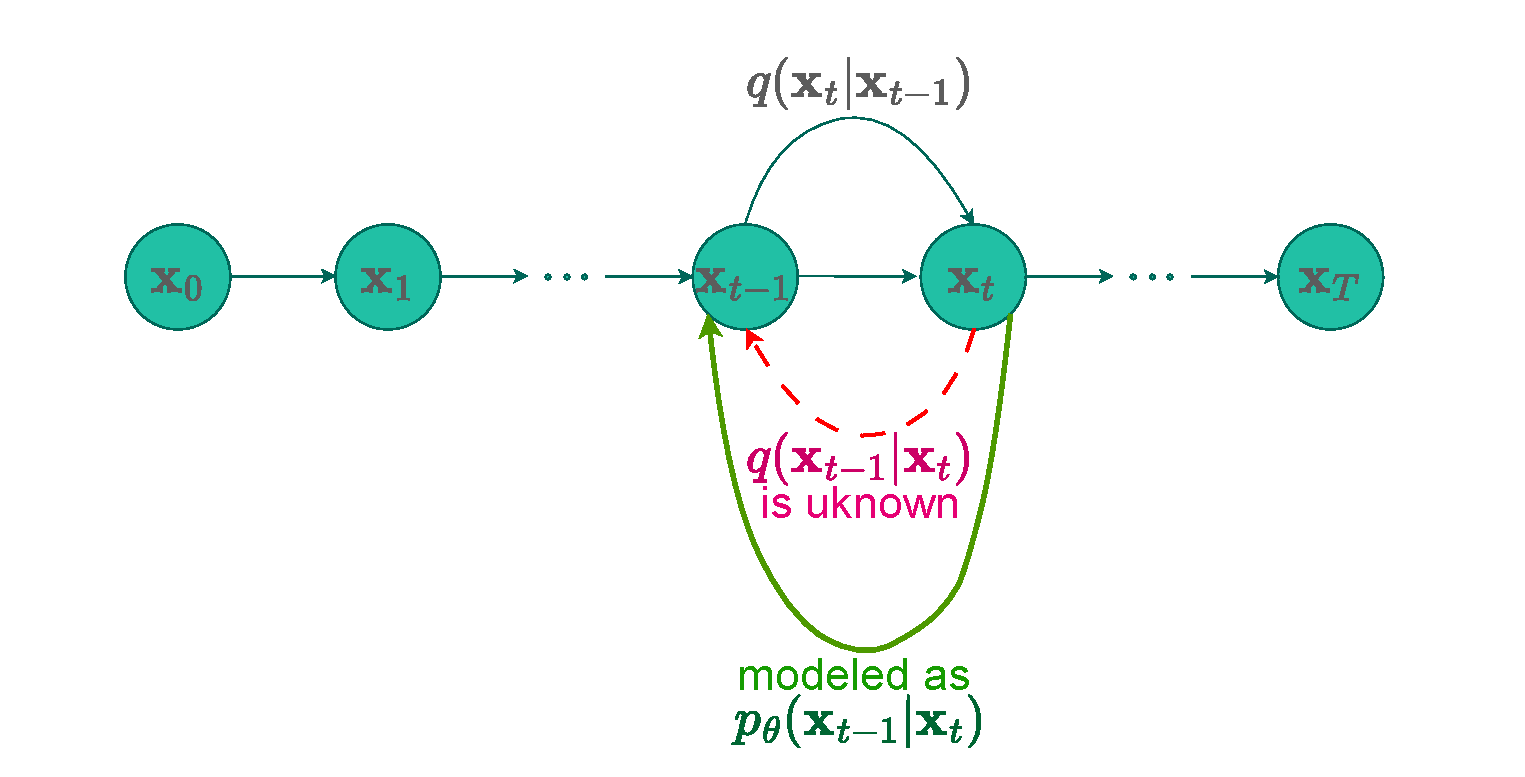
\includegraphics[width=0.99\textwidth, trim={0 0 0 0}, clip]{figures/Diffusion_Model_Reverse_Process.pdf}
              \end{center}
    \end{frame}
    
    \begin{frame}{Reverse Diffusion Process: Removing Noise}
    \begin{itemize}
        \item We need to learn a model $p_\theta$ to approximate these conditional probabilities $q(\xbf_{t-1}|\xbf_t)$  to run the reverse diffusion process.
        \item We start with choosing the prior distribution $p(\xbf_T) = \Ncal(\xbf_T; 0, \Ibf)$ (because in forward process, we end up with $q(\xbf_T)\approx \Ncal(\xbf_T; 0, \Ibf)$.
        \item The learnable transition kernel $p_\theta(\xbf_{t-1}|\xbf_t)$ can be obtained using a neural network model.
        \item The learnable transition kernel can be mathematically written as a parametrized equation
        $$
        p_\theta(\xbf_{t-1}|\xbf_t) = \Ncal(\xbf_{t-1};\bm\mu_\theta (\xbf_t, t), \bm\Sigma_\theta (\xbf_t, t)).
        $$
        $\bm\mu_\theta$ and $\bm\Sigma_\theta$ are parameters to be learned using a neural network (UNet).  An easier option is to set $\bm\Sigma_\theta (\xbf_t, t) = \sigma_t^2 \Ibf$.
        
        \item With this reverse Markov chain in hand, we can generate a data sample $\xbf_0$ by first sampling a noise vector $\xbf_T \sim p(\xbf_T )$, then iteratively sampling from the learnable
    transition kernel $x_{t-1} \sim p_\theta(\xbf_{t-1}|\xbf_t)$ until $t = 1$.
    \end{itemize}
    \end{frame}
    
    
    \begin{frame}{Data Scaling}
    
    \footnotesize
    
    \begin{itemize}
    \item Image data are between 0 to 255 in integer. We scale them to $[-1, 1]$.
    \item Since, image pixels are discrete, we want to obtain discrete log likelihood.
    \item For that, we set the last term of the reverse process to an independent discree decoder derived from the Gaussian $\Ncal(\xbf_0, \bm\mu_\theta (\xbf_1, 1), \sigma_1^2\Ibf)$:

\begin{align*}
p_\theta = \prod_{i=1}^D \int_{\delta_{-}(x_0^i)}^{\delta_{+}(x_0^i)} \Ncal(x; \mu_\theta^i (\xbf_1, 1), \sigma_1^2) dx \quad D \text{ is the data dimensionality} 
\end{align*}  

and

\begin{align*}
\delta_+(x) = \begin{cases}
\infty \quad \text{ if } x = 1\\
x + \frac{1}{255} \quad \text { if } x < 1
\end{cases}
\end{align*}  
 
\begin{align*}
\delta_-(x) = \begin{cases}
-\infty \quad \text{ if } x = -1\\
x - \frac{1}{255} \quad \text { if } x > -1
\end{cases}
\end{align*}  
    
    \end{itemize}
    
    \end{frame}
    
    \begin{frame}{What about the Loss Function?}
        \begin{itemize}
            \item The primary objective in training the UNet is the reverse Markov chain to match the
    actual time reversal of the forward Markov chain.
    \item We need to adjust the parameter $\theta$ in such a way so that joint probability distribution of the reverse Markov chain $p_\theta(\xbf_0,\xbf_1, \cdots,\xbf_T) = p(\xbf_T)\prod_{i=1}^T p_\theta (\xbf_{t-1}|\xbf_t)$ should closely approximate of the forward process $q_\theta(\xbf_0,\xbf_1, \cdots,\xbf_T) = q(\xbf_0)\prod_{i=1}^T q_\theta (\xbf_{t}|\xbf_{t-1})$.
    \item This is done by minimizing the distance between these two joint probability distributions using \textbf{Kullback-Leibler (KL) divergence}.
        \end{itemize}
    \end{frame}
    
    \begin{frame}{KL Divergence as Loss Function}
        \begin{itemize}
            \item KL divergence for training the diffusion model is written as
                \begin{align*}
                      \text{KL}(q, p) & = -\Ebb_{q(\xbf_0,\xbf_1, \cdots,\xbf_T)} [\log p_\theta(\xbf_0,\xbf_1, \cdots,\xbf_T)] + \text{constant}\\
                      & = \Ebb_{q(\xbf_0,\xbf_1, \cdots,\xbf_T)}\bigg[ -\log p(\xbf_T) - \sum_{t=1}^T\log \cfrac{p_\theta(\xbf_{t-1}| \xbf_t)}{q(\xbf_{t}| \xbf_{t-1})} \bigg] + \text{constant}\\
                      & \geq \Ebb_{q(\xbf_0)}[-\log p_\theta(\xbf_0)] + \text{constant} 
                \end{align*}
          The last inequality comes from Jensens's Inequality, i.e. 
    
          $$
          \Ebb[g(X)] \geq g( \Ebb[X] )
          $$
          
          
        \end{itemize}
        
        $\Ebb_{q(\xbf_0}[-\log p_\theta(\xbf_0)]$ is variational upper bound (or negative ELBO as seen in VAE).
        
        \begin{center}
        \tiny

        Two random variables $A$ and $B$ are related by $P(A, B) = P(A) P (B|A)$. Hence,  $q(\mathbf{x}_0, \mathbf{x}_{1:T}) = q(\mathbf{x}_0) q(\mathbf{x}_{1:T} | \mathbf{x}_0)$ which can be used as alternative expression above.
        
        \end{center}
    \end{frame}
    
    \begin{frame}{Parametrizing the Loss Function}
    
    We can rewrite $KL$ shown previously as 
    
    \begin{align*}
    \Ebb_{q(\xbf_0,\xbf_1, \cdots,\xbf_T)}\bigg[\underbrace{KL( q(\xbf_T | \xbf_0) || p(\xbf_T) )}_{L_T} + \sum_{t > 1} \underbrace{KL( q(\xbf_{t-1} | \xbf_t, \xbf_0) || p_\theta(\xbf_{t-1} | \xbf_t))}_{L_{t-1}} \underbrace{- \log p_\theta(\xbf_0 | \xbf_1)}_{L_0} \bigg]
    \end{align*}
    
    This equation uses KL divergence to directly compare $p_\theta(\xbf_{t-1} | \xbf_t)$ against forward process posteriors $q(\xbf_{t-1} | \xbf_t, \xbf_0)$ which are tractable when conditioned on $\xbf_0$:
    \begin{align*}
    q(\xbf_{t-1} | \xbf_t, \xbf_0)  = \Ncal(\xbf_{t-1}; \tilde{\mu}(\xbf_t, \xbf_0), \tilde{\beta}_t \Ibf)
    \end{align*}
    
    with $\tilde{\mu}(\xbf_t, \xbf_0):= \frac{\sqrt{\bar{\alpha}_{t-1}}\beta_t}{1- \bar{\alpha}_t}\xbf_0 + \frac{\sqrt{1 - \beta_t}(1  - \bar{\alpha}_{t-1})}{1 - \bar{\alpha}_t}\xbf_t$ and $\tilde{\beta}_t : = \frac{1- \bar{\alpha}_{t-1}}{1- \bar{\alpha}_t}\beta_t$.
    
    \end{frame}
    
        \begin{frame}{Parametrizing the Loss Function}
        
        \footnotesize

Both $q(\xbf_{t-1} | \xbf_t, \xbf_0)$ and $p_\theta(\xbf_{t-1}| \xbf_t)$ are not Normal distribution, leading to a simpler KL divergence:
\begin{align*}
L_{t-1} = KL( q(\xbf_{t-1} | \xbf_t, \xbf_0) || p_\theta(\xbf_{t-1}| \xbf_t)) = \Ebb_q \bigg [ \frac{1}{2\sigma^2_t} || \tilde{\mu_t}(\xbf_t, \xbf_0) - \mu_\theta (\xbf_t, t) || ^2 \bigg] + C
\end{align*}

We already have one reparameterization: $\xbf_t = \sqrt{\bar{\alpha}_t}\xbf_0 + \sqrt{(1-\bar{\alpha}_t)}\epsilon$.

Then,

\begin{align*}
\tilde{\mu}(\xbf_t, \xbf_0) = \frac{1}{\sqrt{1 - \beta_t}} \bigg( \xbf_t - \frac{\beta}{\sqrt{1 - \bar{\alpha}_t}}\epsilon \bigg)
\end{align*}

So the mean of denoising model can be learnt with a denoising network 

\begin{align*}
\mu_\theta(\xbf_t, t) = \frac{1}{\sqrt{1 - \beta_t}} \bigg( \xbf_t - \frac{\beta}{\sqrt{1 - \bar{\alpha}_t}} \epsilon_\theta(\xbf_t, t) \bigg)
\end{align*}
        
        \end{frame}

\begin{frame}{Simplified Loss Function}

With the parameterization, we have

\begin{align*}
L_{t-1} = \Ebb_{\xbf_0 \sim q(\xbf_0), \epsilon\sim \Ncal(0,\Ibf) }\bigg[ \underbrace{\frac{\beta_t^2}{2\sigma_t^2(1 - \beta_t)(1-\bar{\alpha}_t)}}_{\lambda_t} || \epsilon - \epsilon_\theta(\xbf_t, t)||^2 \bigg] + C
\end{align*}

The time dependent $\lambda_t$ enables the training objective to be weighted for the maximum data likelihood training.

\vspace{10pt}

The original paper simplifies even further, and set $\lambda_t = 1$, and hence


\begin{align*}
L_{simple} = \Ebb_{\xbf_0 \sim q(\xbf_0), \epsilon\sim \Ncal(0,\Ibf) }\bigg[ || \epsilon - \epsilon_\theta(\xbf_t, t)||^2 \bigg] + C
\end{align*}


\end{frame} 

\newcommand{\redbox}[1]{%
  \tikz[baseline=(char.base)]
  \node[draw=red, rectangle, inner sep=2pt, thick] (char) {#1};
}

\begin{frame}{Training and Sample Generation Algorithm}

\begin{columns}[t]
        % Left Column: Training
        \begin{column}{0.5\textwidth}
            \textbf{Algorithm 1} Training
            \hrule
            \begin{algorithmic}[1]
                \REPEAT
                \STATE $\mathbf{x}_0 \sim q(\mathbf{x}_0)$
                \STATE $t \sim \text{Uniform}(\{1, \dots, T\})$
                \STATE $\boldsymbol{\epsilon} \sim \mathcal{N}(\mathbf{0}, \mathbf{I})$
                \STATE Take gradient descent step on
                \STATE $\nabla_\theta \left\| \boldsymbol{\epsilon} - \boldsymbol{\epsilon}_\theta(\redbox{$\sqrt{\bar{\alpha}_t}\mathbf{x}_0 + \sqrt{1 - \bar{\alpha}_t}\boldsymbol{\epsilon}$}, t) \right\|^2$
                \UNTIL{converged}
            \end{algorithmic}
            \hrule
        \end{column}

        % Right Column: Sampling
        \begin{column}{0.5\textwidth}
            \textbf{Algorithm 2} Sampling
            \hrule
            \begin{algorithmic}[1]
                \STATE $\mathbf{x}_T \sim \mathcal{N}(\mathbf{0}, \mathbf{I})$
                \FOR{$t = T, \dots, 1$}
                \STATE $\mathbf{z} \sim \mathcal{N}(\mathbf{0}, \mathbf{I})$
                \STATE \redbox{$\mathbf{x}_{t-1} = \frac{1}{\sqrt{\alpha_t}} \left( \mathbf{x}_t - \frac{1-\alpha_t}{\sqrt{1-\bar{\alpha}_t}} \boldsymbol{\epsilon}_\theta(\mathbf{x}_t, t) \right)$} $+ \sigma_t \mathbf{z}$
                \ENDFOR
                \RETURN $\mathbf{x}_0$
            \end{algorithmic}
            \hrule
        \end{column}
    \end{columns}
    

\end{frame}   
    
    %------------------------------------------------
    \section{Latent Diffusion Models}
    %------------------------------------------------
    
    %------------------------------------------------
    \begin{frame}{}
    \begin{center}
        \huge \bf \color{DarkBlue}
        Latent Diffusion Models
    \end{center}
    \end{frame}
    
    \begin{frame}{Latent Diffusion Model}
        \begin{center}
        {\large \bf \color{MediumBlue}
            The diffusion model runs in a latent space instead of a pixel space, making training costs lower and inference faster.
        }
        
        \vspace{15pt}
        
        Latent: hidden or compression space (like PCA)!
        
        \vspace{15pt}
        
    
        {\large \bf \color{MediumRed}
            One example of the Latent Diffusion Model is StableDiffusion (the one that lets you generate images from the text).
        }
        
        \end{center}    
    \end{frame}
    
    \begin{frame}{Latent Diffusion Model Architecture}
        \begin{center}
            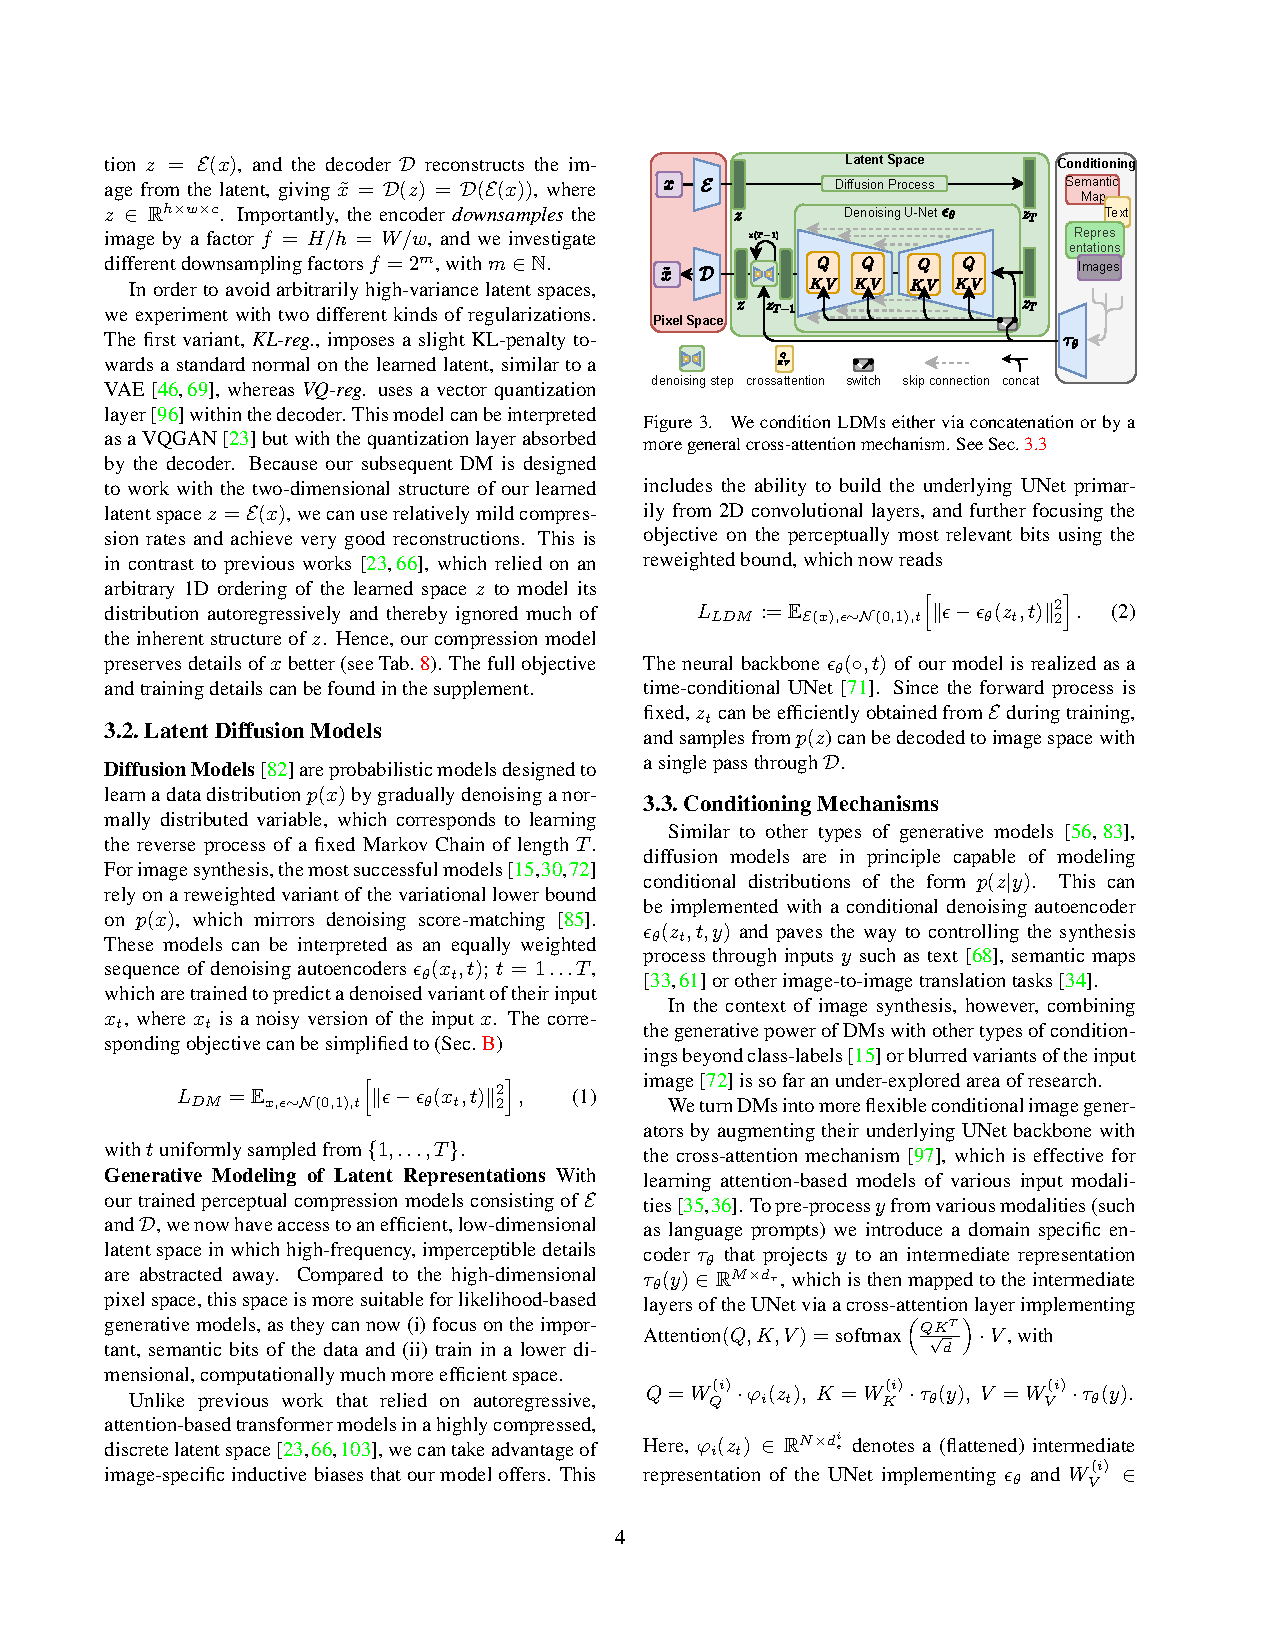
\includegraphics[width=0.87\textwidth, trim={300 600 50 70}, clip]{figures/LatentDiffusionModel.pdf}
        \end{center}
    \end{frame}

    
    \begin{frame}{Code Demo}
        \begin{center}
            {\large \bf\color{MediumGreen} UNet Diffusion Model on Fashion MNIST Dataset: \url{https://github.com/rahulbhadani/CPE487587_SP26/blob/master/Code/Chapter_08_DiffusionModel.ipynb}
            }
    
    \vspace{20pt}
            
    {\large \bf\color{MediumBlue} UNet Diffusion Model on Digit MNIST Dataset: \url{https://colab.research.google.com/drive/1RqgzkjEL-W3lUOhUkzAoEcVlnM0Cu1Fp?usp=sharing}
    }
        \end{center}
    \end{frame}
    

  %------------------------------------------------
    \section{ODE, Flow, and Dynamical Systems}
    %------------------------------------------------
    
    %------------------------------------------------
    \begin{frame}{}
    \begin{center}
        \huge \bf \color{DarkBlue}
        ODE, Flow, and Dynamical Systems
    \end{center}
    \end{frame}    
    
    
    \begin{frame}{Ordinary Differential Equations}
    
    A first order ODE:
    
    \begin{align*}
    y'(t) = \frac{dy}{dt} = f(t, y(t))
    \end{align*}
    with initial condition $y(0) = y_0$.
    
    In general, an ODE is a functional relation of the form 
    
    \begin{align*}
    F(t, x, x^{(1)}, \cdots, x^{(k)}) = 0
    \end{align*}

where $x^{(j)}(t) = \frac{d^j x(t)}{dt^j}$ the j-th derivative.

\vspace{5pt}

$t$ is called the independent variable, and $x$ is the dependent variable. The highest derivative is the order of the ODE.
    
    \end{frame}
    
    \begin{frame}{A System of ODE}
    
    \begin{align*}
    x_1^{(k)}&  = f_1(t, x, x^{(1)}, \cdots, x^{(k-1)}\\
    x_2^{(k)}&  = f_2(t, x, x^{(1)}, \cdots, x^{(k-1)}\\
    \vdots\\
    x_n^{(k)}&  = f_n(t, x, x^{(1)}, \cdots, x^{(k-1)}\
    \end{align*}
    
    \end{frame}
    
    \begin{frame}{A linear system of ODE}
    
    A system of ODE is linear if it is of the form 
    
    \begin{align*}
    x_i^{(k)} = g_i(t) + \sum_{i=1}^n \sum_{j=0}^{k-1} f_{i,j,l} (t) x_l^{(j)}
    \end{align*}
    
    Further, it is \textbf{homogenous} if $g_i(t) = 0$.
    
    \end{frame}
    
    \begin{frame}{First-order ODE System}

\begin{columns}

\column{0.5\linewidth}

    
    Any system can always be reduced to a first-order system by
changing to the new set of dependent variables $y = (x, x^{(1)}, \cdots , x^{(k-1)}$ which yields

\begin{align*}
\ydot_1 & = y_2\\
\ydot_2 & = y_3\\
\vdots\\
\ydot_{k-1} & = y_k\\
\ydot_k & = f(t,y)
\end{align*}

\pause

\column{0.5\linewidth}



We can even add $t$ to the dependent variables $z = (t,y)$, making the right hand side independent of $t$. Hence

\begin{align*}
\zdot_1 &  = 1\\
\zdot_2 & = z_3\\
\vdots\\
zdot_k & = z_{k+1}\\
\zdot_{k+1} & = f(z)
\end{align*}

Such a system where $f$ does't depend on $t$ is called \textbf{autonomous} system.


\end{columns}    


    \end{frame}
    
    \begin{frame}{Firsr-order Autonomous Equations}
    
    The solution starting at a certain point $x_0$ at
time $t = 0$ is
    
    \begin{align*}
    \xdot = f(x), \quad x(0) = x_0
    \end{align*}
    
    It is also called \textbf{Initial Value Problem}.
    
    We can have a solution $\phi(t)$ with $\phi(0) = x_0$ and the solution $\psi(t)$ with $\psi(t_0) = x_0$ for a general time $t_0$ is given by a simple shift $\psi(t) = \phi(t-t_0)$. This holds for any autonomous equation.
    
    \end{frame}

\begin{frame}{Dynamical Systems}

\footnotesize

\begin{tcolorbox}
Think of a dynamical system as the time evolution of some physical
system, such as the motion of a few planets under the influence of their
respective gravitational forces
\end{tcolorbox}

\vspace{6pt}

Usually we want to know the fate of such a system for long times, like will planet eventually collide or will the system persist for all times?

\vspace{6pt}

Such analysis is embedded in \textbf{dynamical systems theory}. A dynamical system is a map

\begin{align*}
T: G\times M \to M
\end{align*}

$M$ is a set and $G = \Nbb_0$ or $G = \Zbb$ for discrete dynamical system and $G = \Rbb$ for a continuous dynamical system.

\vspace{6pt}

\begin{tcolorbox}[colframe=uiRose, title=~~]
The Cauchy-Peano theorem, and The Picard-Lindelöf theorem  imply that for continuously differentiable dynamical systems,  there is a unique solution to every initial value problem.
\end{tcolorbox}

\scriptsize

A refersher on ODE: \url{https://opentextbooks.library.arizona.edu/mathematicalmodeling/chapter/appendix-ordinary-differential-equations/}



\end{frame}    


\begin{frame}{The Flow of An Autonomous Equation}

    \small

Let's look at an autonomus system

\begin{tcolorbox}[
    enhanced,
    sharp corners,
    % Set the base thickness for all sides
    boxrule=1pt, 
    % Specifically override the left side
    leftrule=2mm, 
    % Colors
    colframe=vcGold,
    colback=WarmWhite,
    % Ensure no title space is reserved
    notitle,
    % Optional: Add some padding so text doesn't touch the thick edge
    left=2mm 
]
\begin{align*}
    \xdot = f(x), \quad x(0) = x_0, x \in \Rbb^n, \quad f:\Rbb^n \to \Rbb^n
\end{align*}
\end{tcolorbox}

Here, we say that the solution doesn't depend on the time (autonomous equation).

\begin{tcolorbox}[
    enhanced,
    sharp corners,
    % Set the base thickness for all sides
    boxrule=1pt, 
    % Specifically override the left side
    leftrule=1mm, 
    % Colors
    colframe=Rust,
    colback=white,
    % Ensure no title space is reserved
    notitle,
    % Optional: Add some padding so text doesn't touch the thick edge
    left=2mm 
]
The solution starting from $x_0$ at time $t = 0$ is a curve $t \mapsto \varphi_t(x_0)$ satisfying $\frac{d}{dt}\varphi_t(x_0) = f(\varphi_t(x_0))$ and $\varphi_0(x_0) = x_0$.
\end{tcolorbox}

\textbf{\underline{Definition of Flow:}} {\color{mainNavy} The flow of the ODE is the family of maps $\varphi: \Rbb \times \Rbb^n \to \Rbb^n$, $(t, x_0) \mapsto \varphi(x_0)$.}


\end{frame}

\begin{frame}{The Flow of an Autonomous Equation}


\begin{center}
    \begin{tcolorbox}[colback=softblue, colframe=mainblue, arc=4pt, boxrule=1pt, left=10pt, right=10pt, top=8pt, bottom=8pt]
    Rather than finding specific solution, the flow allows to examine the behavior of solutions to an IDE at a 'larger scale' qualitatively.

    \vspace{10pt}

    We track ensemble of solutions emnating from a set of points all at the same time.
    \end{tcolorbox}

    \vspace{10pt}

    \footnotesize
    {

    \color{roseRed!50!black}

    A related concept is diffeomorphism, where you can understand two sheet of papers, and distort one sheet, and you can still establish mappings from one sheet of paper to another sheet. Hence, essentially you cam say that $\varphi_t: \Rbb^n \to \Rbb^n$ is a flow, which is a diffeomorphism for each fixed $t$ and is a deformation of state space that \textit{transports} every point along its trajectory for time $t$.

    }

    \vspace{5pt}

    Let's look at an animation: 
    
    \url{https://aarc-lab.github.io/animation/ode_diffeomorphism_deformed_grid.html} 

    \url{https://aarc-lab.github.io/animation/transport_equation_flow.html}

\end{center}
    
\end{frame}

\begin{frame}{An Example of Flow: $\xdot = \sin(x)$}
    
    \begin{center}
        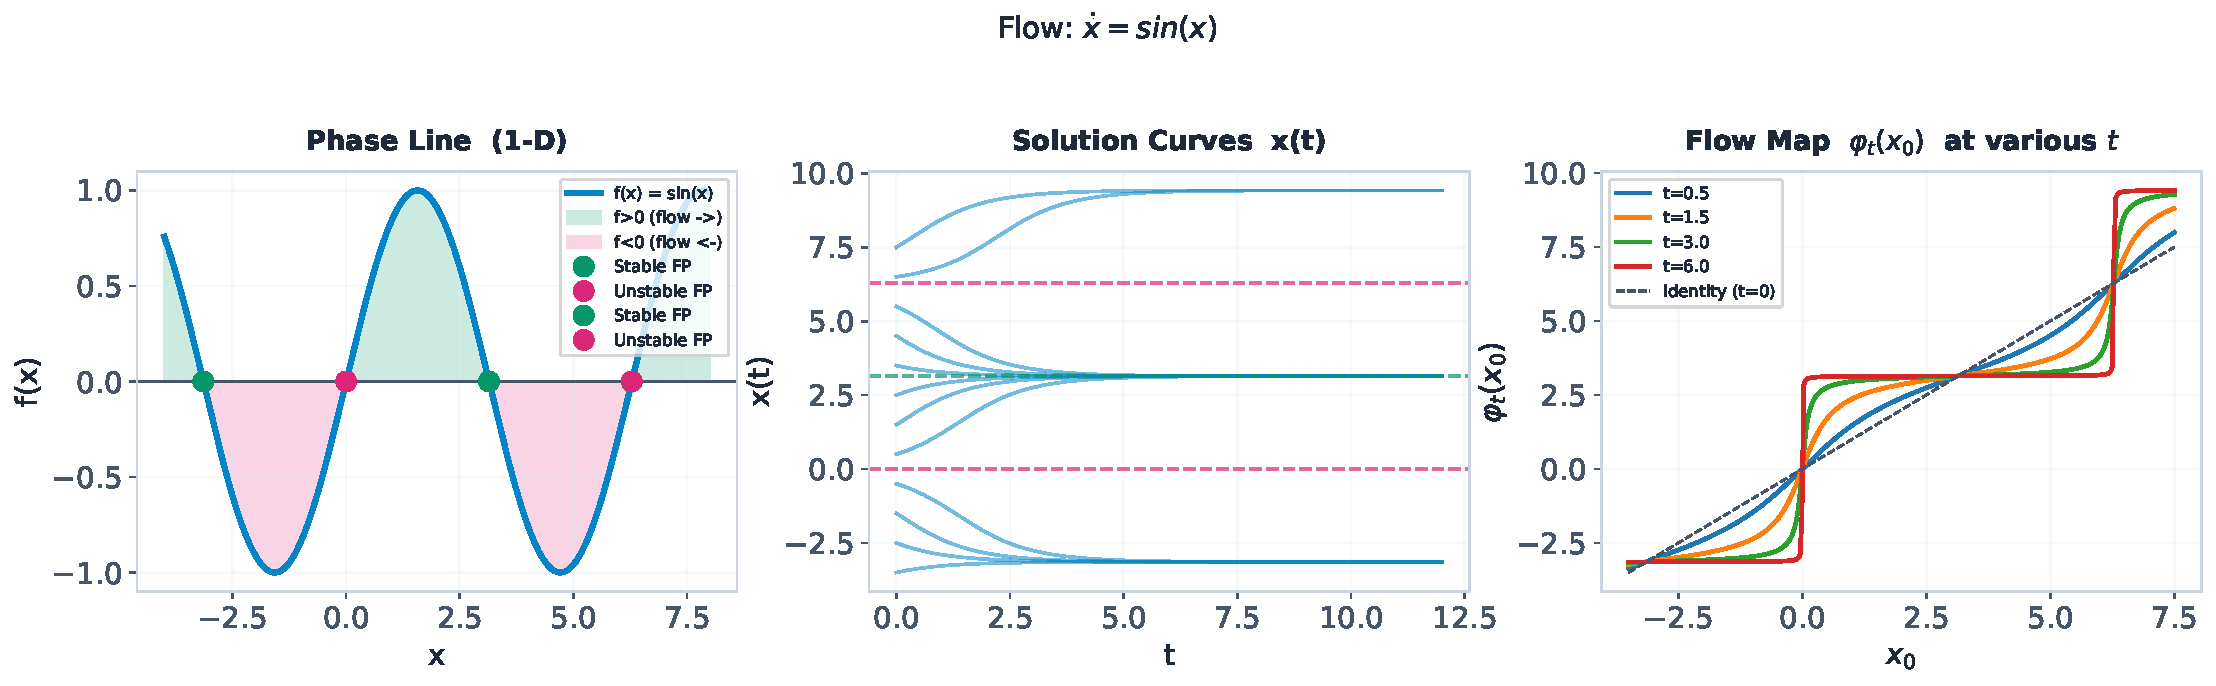
\includegraphics[width=1.0\linewidth, trim={0 0 0cm 0cm},clip]{figures/one_dim_ode_flow_example.pdf}
    \end{center}

    \footnotesize

    {\color{mathGray}The concept of a flow illustrated by $\xdot = \sin(x)$. Left: Phase line showing the 1-D vector field, stable fixed points (green circles, $\cos(x^*)<0$) and unstable fixed points (red circles). Green/red regions indicate flow direction. Center: Solution curves $x(t)$ for different initial conditions, all converging to or diverging from fixed points. Right: The flow map $\varphi_t(x_0)$ at successive times $t=0.5,1.5,3,6$ showing how the identity map deforms into the long-time asymptotics.}

\end{frame}

\begin{frame}{Another Example of Flow}

    \begin{columns}
        \column{0.5\linewidth}

        \begin{align*}
            \dfrac{dy}{dx} = \dfrac{3x^2+4x+2}{2(y-1)}
        \end{align*}

        In 2D, a flow map is visualized through the phase portrait. Each line on the phase portrait corresponds to 

        \column{0.5\linewidth}

                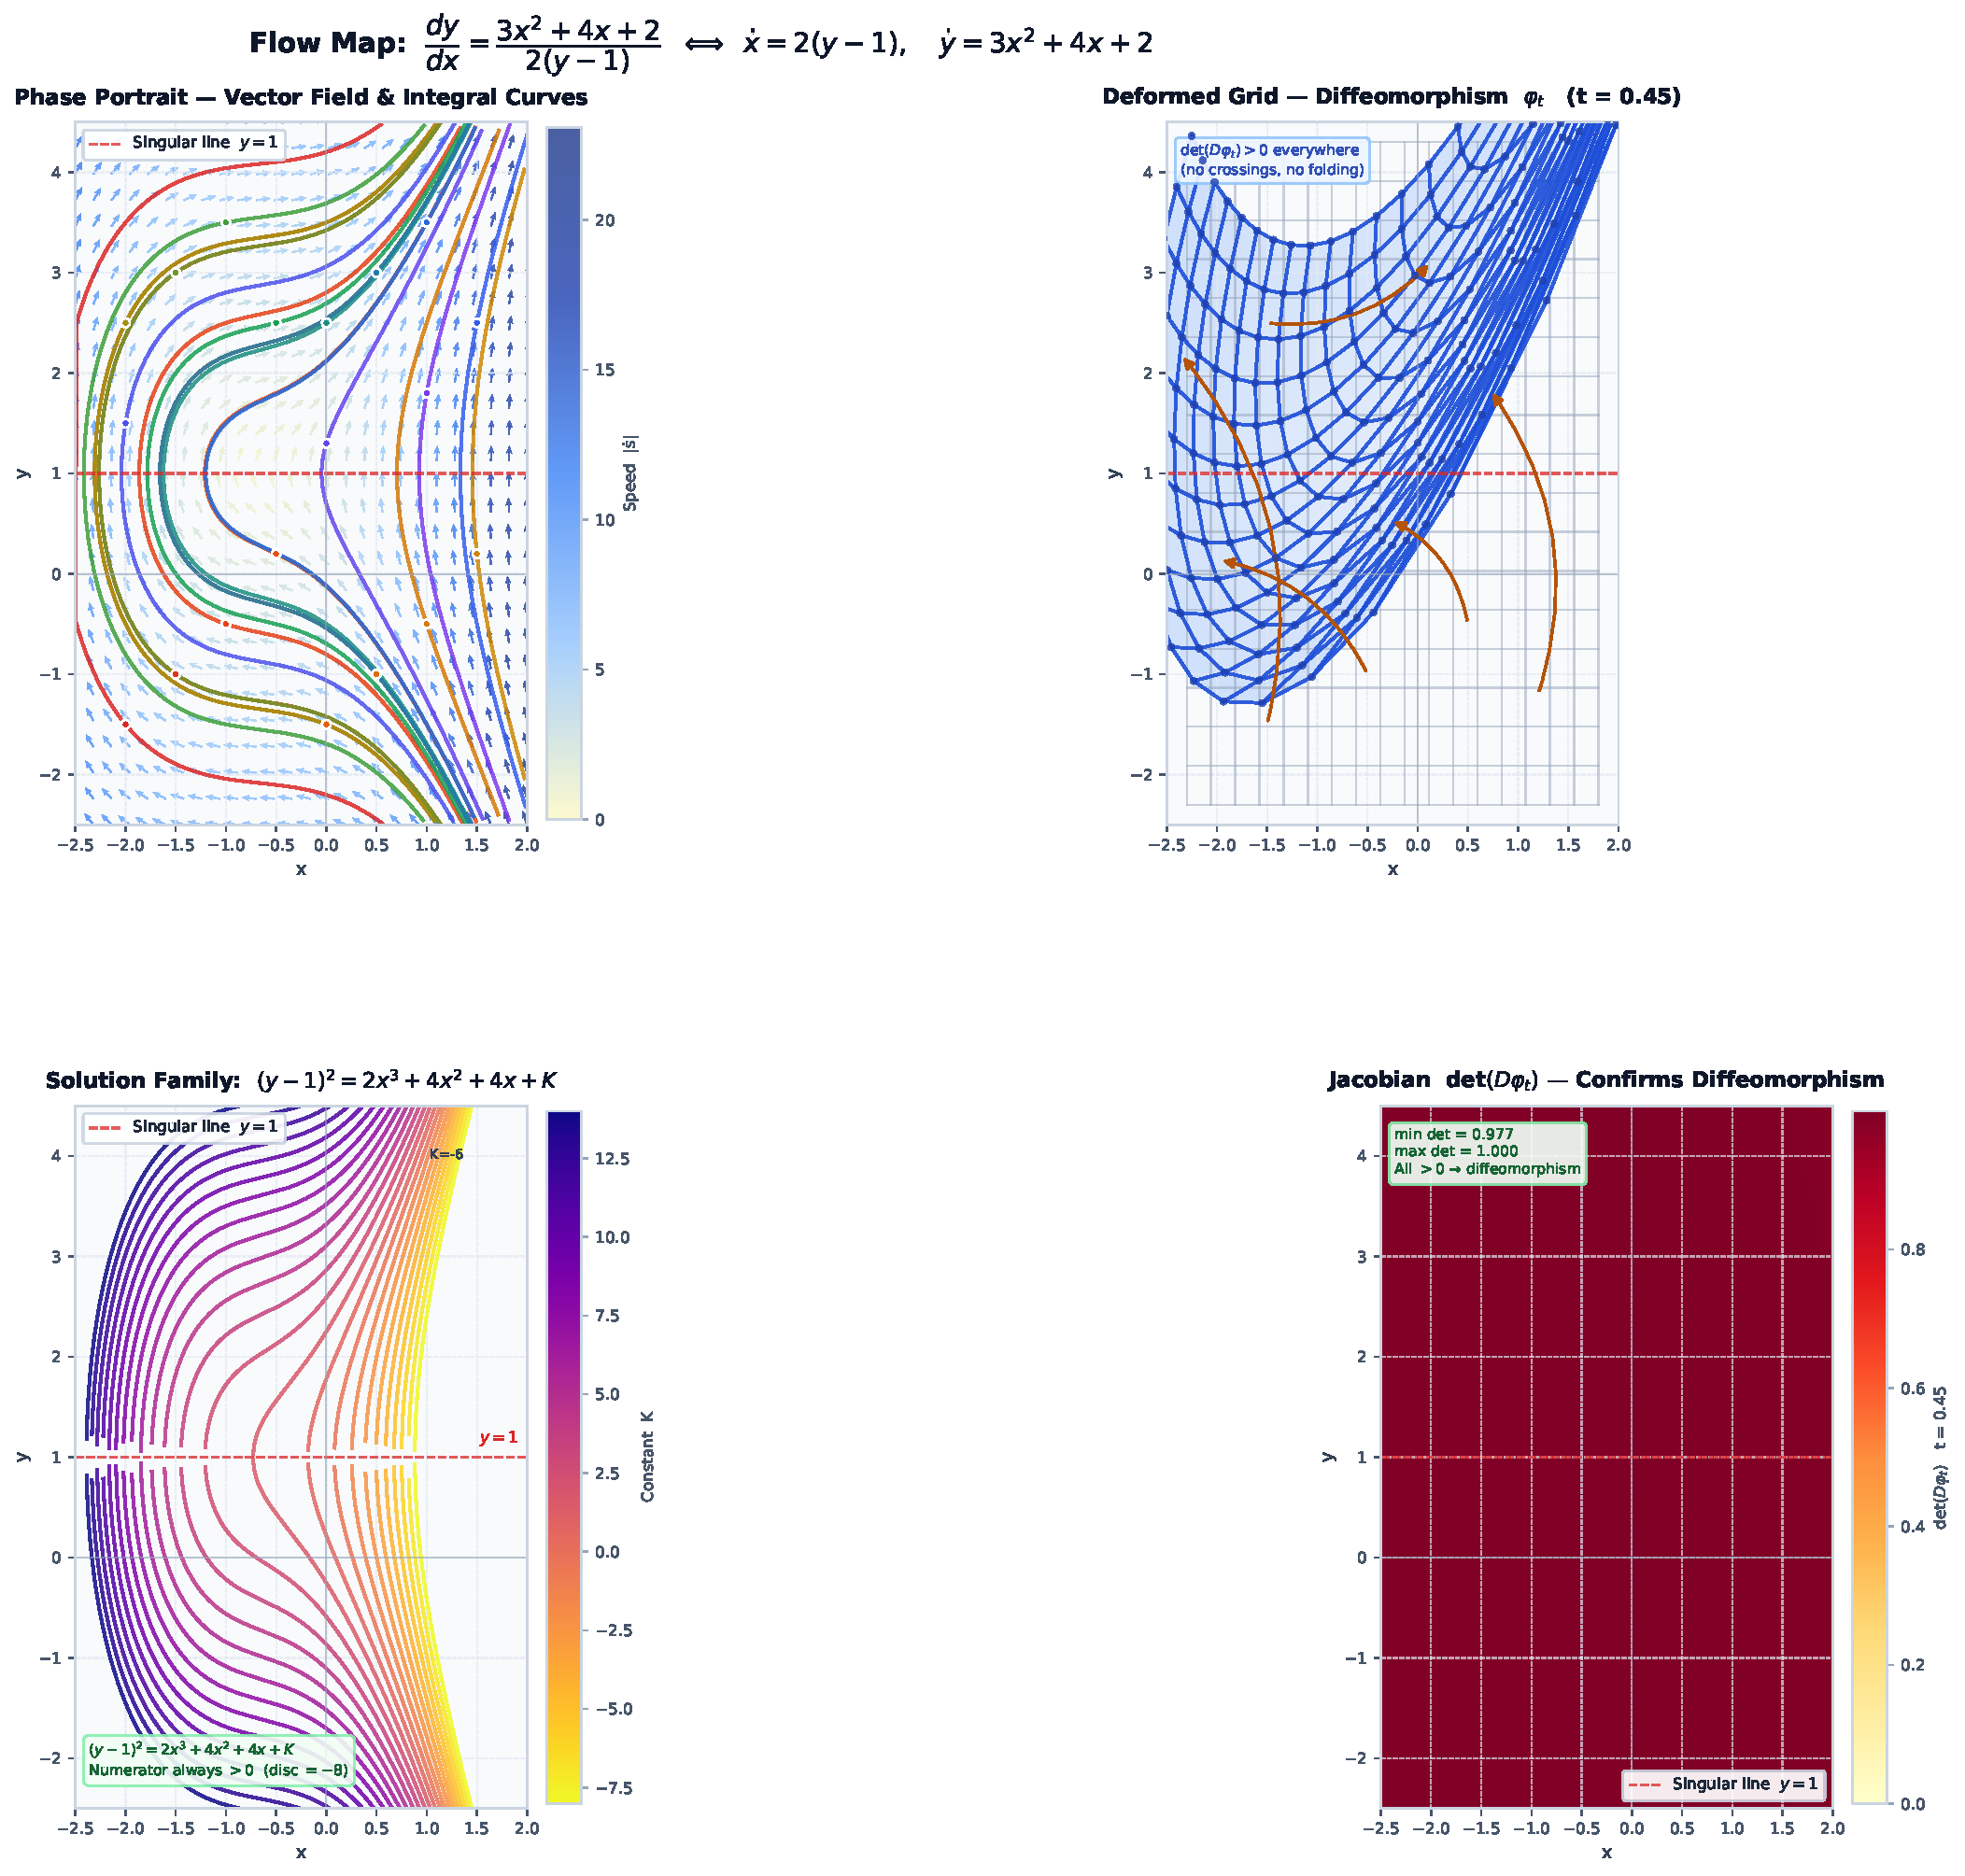
\includegraphics[width=0.75\linewidth, trim={0 15cm 25cm 2cm},clip]{figures/ode_flow_example.pdf}

        
    \end{columns}

\vfill

\end{frame}


\begin{frame}{Linear Systems and Phase Portrait of Its Flow}

\begin{tcolorbox}[vcLight, title=~]
    \color{vcDeep}
A linear system $\xdot = Ax$, where $A \in \Rbb^{n\times n}$ is a matrix, is completely solvable.

\vspace{3pt}

{\scriptsize \url{https://www.ams.org/bookstore/pspdf/gsm-158-prev.pdf}

\url{https://www.nas.nasa.gov/assets/nas/pdf/techreports/1993/rnr-93-003.pdf}

https://www.nas.nasa.gov/assets/nas/pdf/techreports/1993/rnr-93-003.pdf

\vspace{3pt}

$e^A$ is given by Taylor series expansion $e^{A} = \sum_{k=0}^\infty \frac{A^k}{k!}$

\vspace{3pt}

Hence, the flow map is 

\begin{align*}
    \varphi_t(x_0) = e^{At}x_0 = \sum_{k=0}^\infty \frac{A^k}{k!}\cdot x_0
\end{align*}

}
\end{tcolorbox}
\end{frame}
    

\begin{frame}{Behavior of a Linear System through Phase Portrait}

    
    Behavior of a linear system is completely determined by the eigenvalue structure of $A$.

    \vspace{3pt}

    For $n=2$, the eigenvalues are $\lambda_1$, $\lambda_2$ for the matrix $A$.
    
    \vspace{5pt}

    \centering
    \resizebox{0.9\textwidth}{!}
    {
    \begin{tabular}{|p{4.0cm}|p{3.0cm}|p{3.0cm}|p{5.0cm}|p{4.0cm}|}
        \hline
        \textbf{Eigenvalues} & \textbf{Fixed Point} & \textbf{Stability} & \textbf{Phase Portrait} & \textbf{Example} \\ \hline
        $\lambda_1 < \lambda_2 < 0$ & Stable Node & Asymptotically stable & All trajectories $\to$ origin & Overdamped oscillator\\ \hline
        $0 < \lambda_1 < \lambda_2$ & Unstable Node & Unstable & All trajectories $\leftarrow$ origin & Inverted pendulum (near top) \\ \hline
        $\lambda_1 < 0 < \lambda_2$ & Saddle Point & Unstable & Hyperbolic curves & Pendulum near top (nonlinear) \\ \hline
        $\lambda = \alpha \pm j\beta, \alpha < 0$ & Stable Spiral & Asymptotically stable & Inward spirals & Damped oscillator \\ \hline
        $\lambda =  \alpha \pm j\beta, \alpha > 0$ & Unstable Spiral & Unstable & Outward spirals & Amplifier feedback \\ \hline
        $\lambda = \pm j\beta $ & Centre & Lyapunov stable (not asymptotic) & Closed ellipses & Harmonic oscillator \\ \hline
        $\lambda_1 = \lambda_2 < 0$ (distinct eigvec) & Stable Star & Asymptotically stable & Straight lines $\to$ Origin & Critically damped (non-defective) \\ \hline
    \end{tabular}
    }

    
\end{frame}

\begin{frame}{Behavior of a Linear System through Phase Portrait}

    \begin{center}
            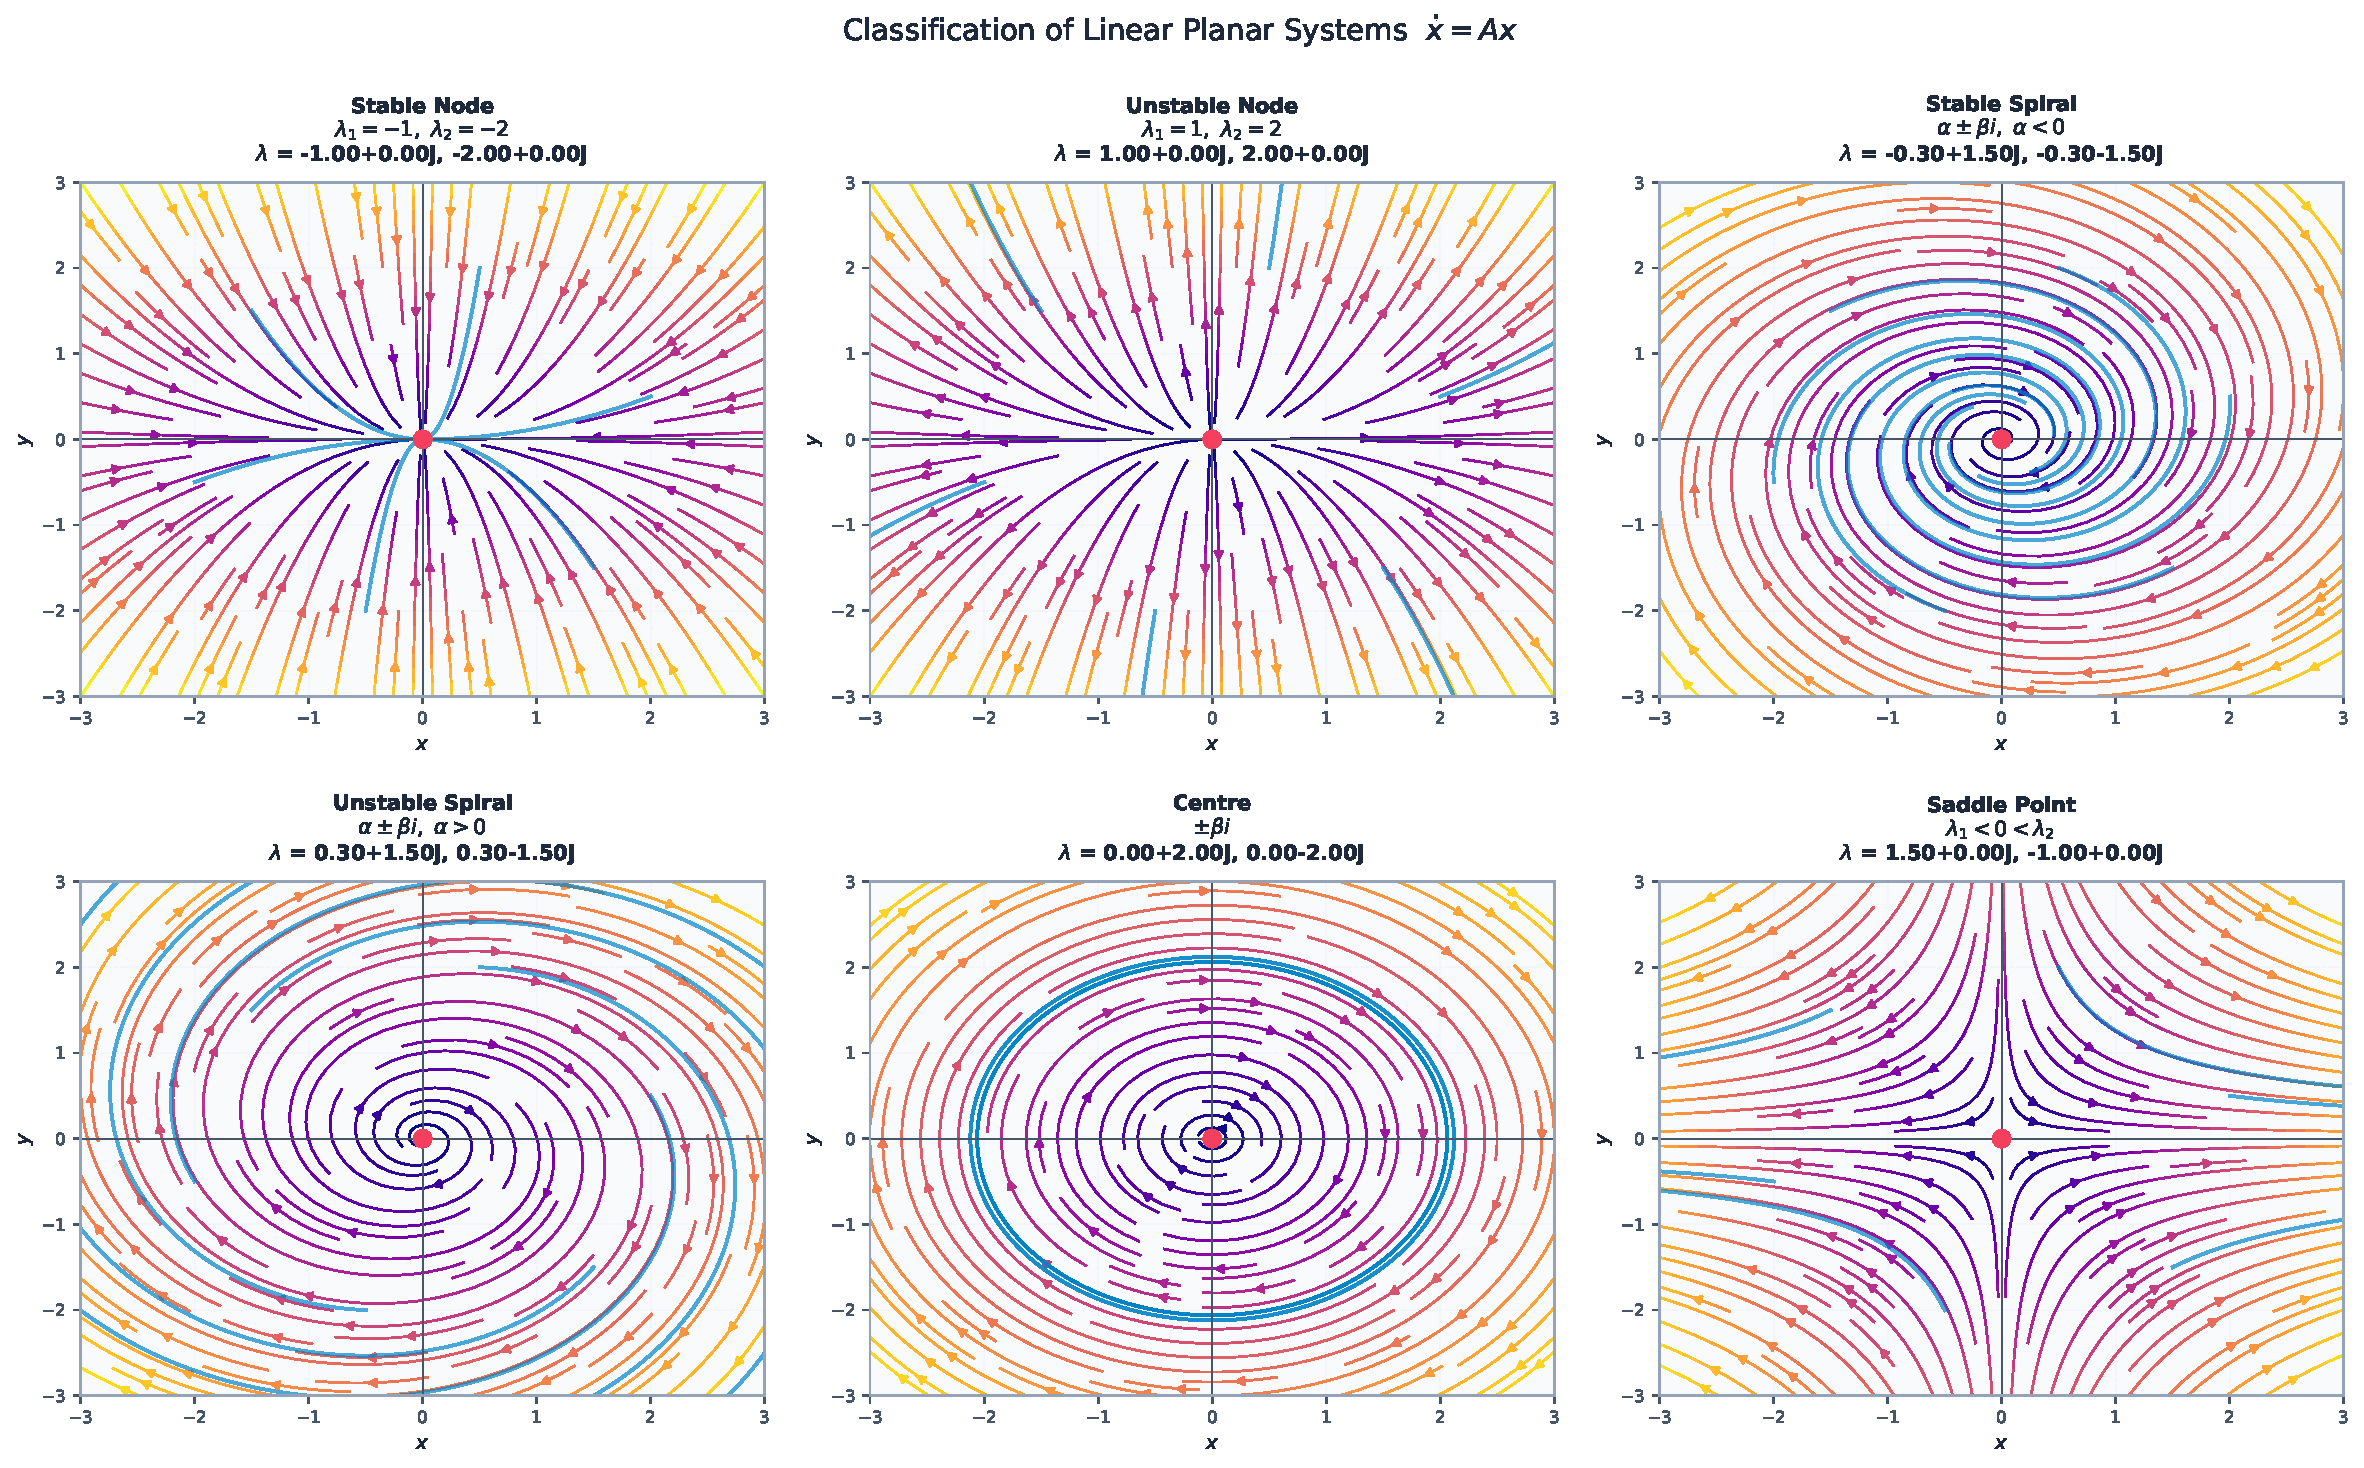
\includegraphics[width=0.75\linewidth, trim={0 0cm 0cm 0cm},clip]{figures/ode_flow_phase_portrait.pdf}
    \end{center}
    
\end{frame}

\begin{frame}{Stability through Lyapunov Function}

    
    $A$ is a stable iff for every $Q>0$, there exists a unique $P>0$ solving

    \begin{tcolorbox}[
        enhanced,
        rounded corners,
        % Set the base thickness for all sides
        boxrule=0.5pt, 
        % Specifically override the left side
        leftrule=2mm, 
        % Colors
        colframe=vcGold!10!purple,
        colback=WarmWhite,
        % Ensure no title space is reserved
        notitle,
        % Optional: Add some padding so text doesn't touch the thick edge
        left=1mm 
    ]
        \begin{align*}
            A^\top  P + PA = -Q
        \end{align*}
    \end{tcolorbox}
    \vspace{10pt}

    The function $V(x) = x^\top P x$ is then a Lyapunov function: $\dot{V} = -x^\top Q x < 0$.

    \vspace{5pt}

    $Q$ is any positive definite matrix (symmetric and all eigenvalues positive).

    \vspace{5pt}

    \scriptsize

    \url{https://eceweb1.rutgers.edu/~gajic/psfiles/LinearLyapunov.pdf}

\end{frame}

\begin{frame}{Nonlinear Systems and Phase Plane Analysis}

    Most physically relevant systems are nonlinear. Although explicit solutions are rarely available, the phase plane (for $n=2$) provides complete qualitative information: fixed points, periodic orbits, separatrices, and the long-time fate of all trajectories.

        \begin{tcolorbox}[
        enhanced,
        rounded corners,
        % Set the base thickness for all sides
        boxrule=0.5pt, 
        % Specifically override the left side
        leftrule=2mm, 
        % Colors
        colframe=vcGold!30!Green,
        colback=WarmWhite,
        % Ensure no title space is reserved
        notitle,
        % Optional: Add some padding so text doesn't touch the thick edge
        left=1mm 
    ]

    A point $x^*$ is a fixed point of $\dot{x} = f(x)$ if $f(x^*) = 0$. The solution starting at $x^*$ remains there forever: $\varphi(x^*) = x^*$ for all $t$.

    \end{tcolorbox}    
\end{frame}

\begin{frame}{Hartman-Grobam Theorem}
    
        \begin{tcolorbox}[
        enhanced,
        rounded corners,
        % Set the base thickness for all sides
        boxrule=0.5pt, 
        % Specifically override the left side
        leftrule=2mm, 
        % Colors
        colframe=orange!80!yellow,
        colback=WarmWhite,
        % Ensure no title space is reserved
        notitle,
        % Optional: Add some padding so text doesn't touch the thick edge
        left=1mm 
    ]

    If $x^*$ is a hyperbolic fixed point (all eigenvalues of Jacobian $Df(x^*)$ have non-zero real part), then the flow of $\xdot = f(x)$ near $x^*$ is topologically conjugate (a qualitative equivalence) to the flow of its linearisation $\xdot = Df(x^*)x$ near the origin. The phase portrait types (node/spiral/saddle) are preserved.
    \end{tcolorbox}
\end{frame}

\begin{frame}{Example: Nonlinear Pendulum}

    \footnotesize

    The pendulum $\ddot{\theta} = -\sin(\theta)$ can be written as a planar system:

    \begin{align*}
        \xdot_1 & = x_2\\
        \xdot_2 & = -\sin(x_1)
    \end{align*}


    \vspace{5pt}


    It has fixed points: $(n\pi, 0)$ for $ n \in \Zbb$. Tha Jacobian is 

    \begin{align*}
        Df(x_1, x_2) = \begin{bmatrix}
            0 & 1\\
            -\cos(x_1) & 0
        \end{bmatrix}
    \end{align*}
    
    \vspace{3pt}

    At $(0,0)$: eigenvalues $\pm j  to ~$ center (for the linearisation; nonlinear analysis confirms it). At $(\pi, 0)$: eigenvalues $\pm 1 \to ~$ saddle point. 

    \vspace{3pt}

    The conserved energy (first integral) is:


            \begin{tcolorbox}[
        enhanced,
        rounded corners,
        % Set the base thickness for all sides
        boxrule=0.5pt, 
        % Specifically override the left side
        leftrule=2mm, 
        % Colors
        colframe=blue!80!red,
        colback=WarmWhite,
        % Ensure no title space is reserved
        notitle,
        % Optional: Add some padding so text doesn't touch the thick edge
        left=1mm 
    ]

    \begin{align*}
    E(\theta, \omega) & = \frac{1}{2} \omega^2 - \cos(\theta) = \text{ constant along trajectories.}    
    \end{align*}
    where $\dot{\theta} = \omega$.
    \end{tcolorbox}
    

\end{frame}

\begin{frame}{Example: Nonlinear Pendulum}

\begin{center}
            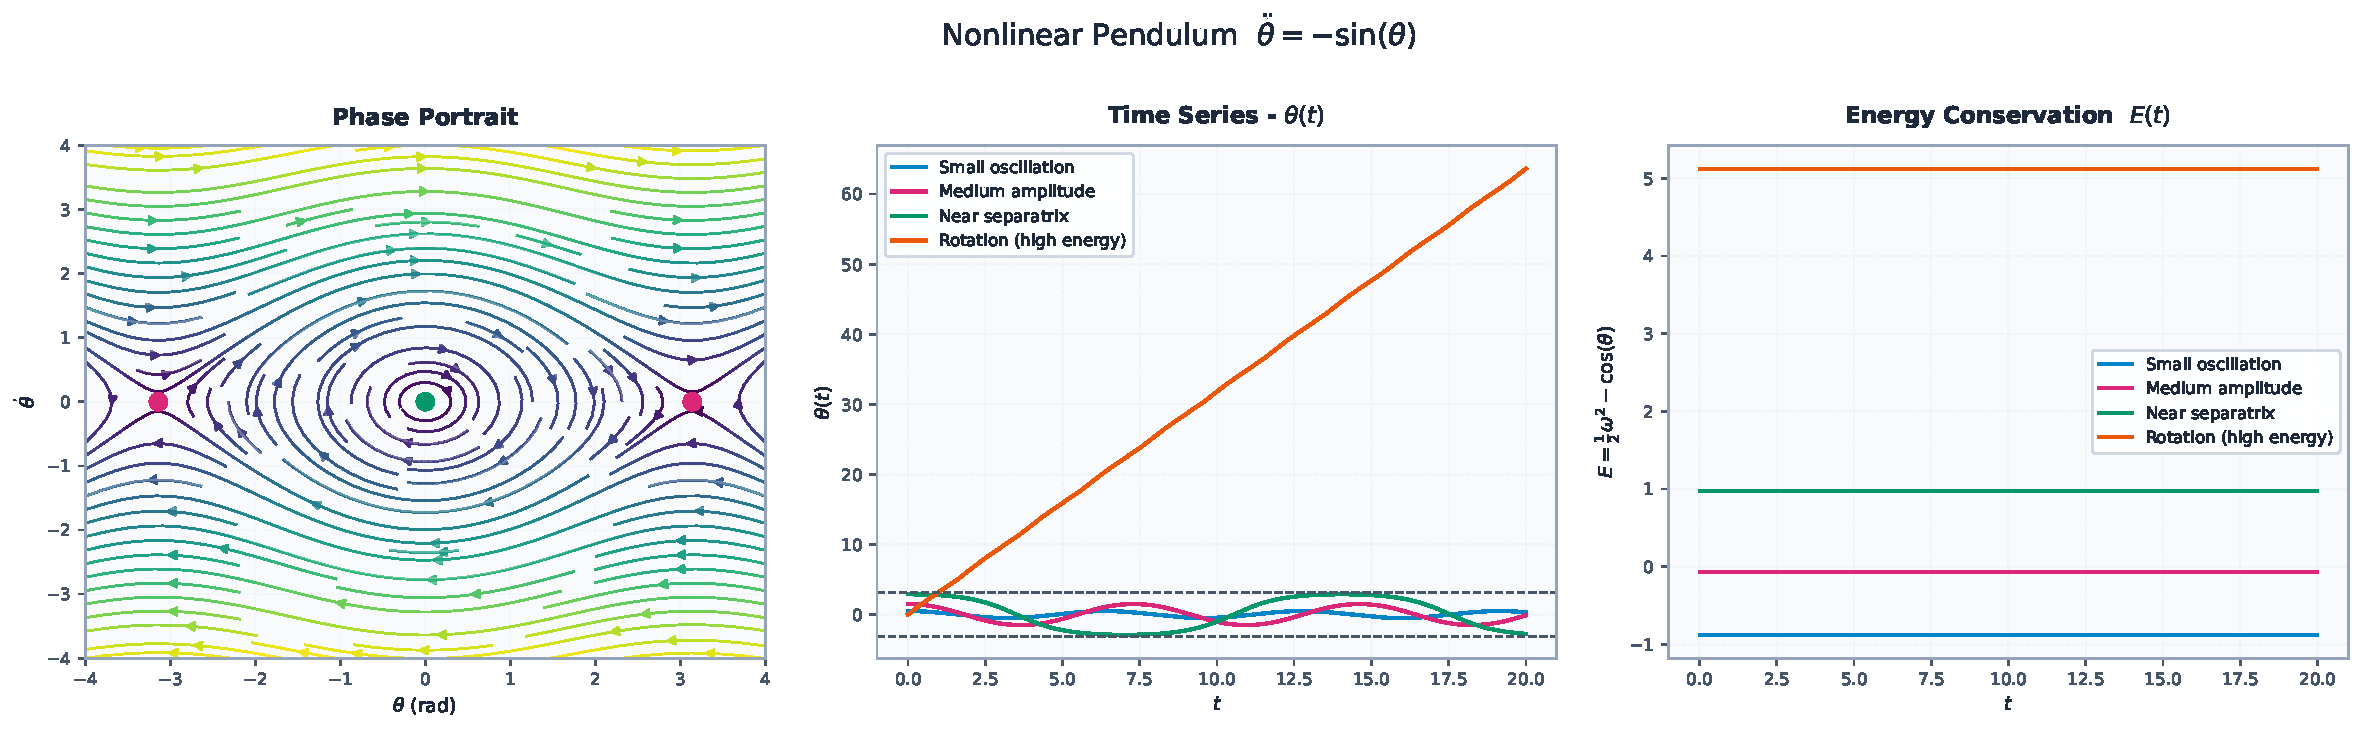
\includegraphics[width=1.0\linewidth, trim={0 0cm 0cm 0cm},clip]{figures/nonlinear_pendulum.pdf}
\end{center}

\footnotesize

    {\color{mathGray}
    \textbf{Left:} Phase portrait with energy contours. Green dots = stable centres (bottom equilibria), red dots = unstable saddles (top equilibria). The separatrix (homoclinic orbit) at $E=1$ separates libration (oscillation) from rotation. \textbf{Center:} Time series for four initial conditions showing qualitatively different regimes. \textbf{Right:} Energy $E(t)$ is conserved (flat lines) confirming the Hamiltonian structure
    }
    
\end{frame}


\begin{frame}{Limit Cycle - Period Orbits in the Plane}
    
    \begin{center}
        
    
    \begin{tcolorbox}[colback=softblue, colframe=mainblue, arc=4pt, boxrule=1pt]

    A limit cycle is an isolated closed orbit in the phase plane. Trajectories from nearby initial conditions spiral toward (stable limit cycle) or away from (unstable) the closed orbit as $t \to \pm \infty$.  Unlike a center, limit cycles have no continuous family of closed orbits surrounding them.

    \end{tcolorbox}
    
    \end{center}

\end{frame}

\begin{frame}{Example: Van der Pol Oscillator}
    
    $$
        \ddot{x} - \mu( 1 - x^2)\xdot + x = 0, \quad \mu > 0
    $$

    \vspace{10pt}

    $-\mu( 1 - x^2)$ acts as negative damping when $|x| < 1$ (pumping energy into oscillation) ad positive damping for $|x| > 1$ (disspating energy). This result in a unique stable limit cycle attracting all non-trivial trajectories.

\end{frame}

\begin{frame}{Example: Van der Pol Oscillator}

    \begin{center}
            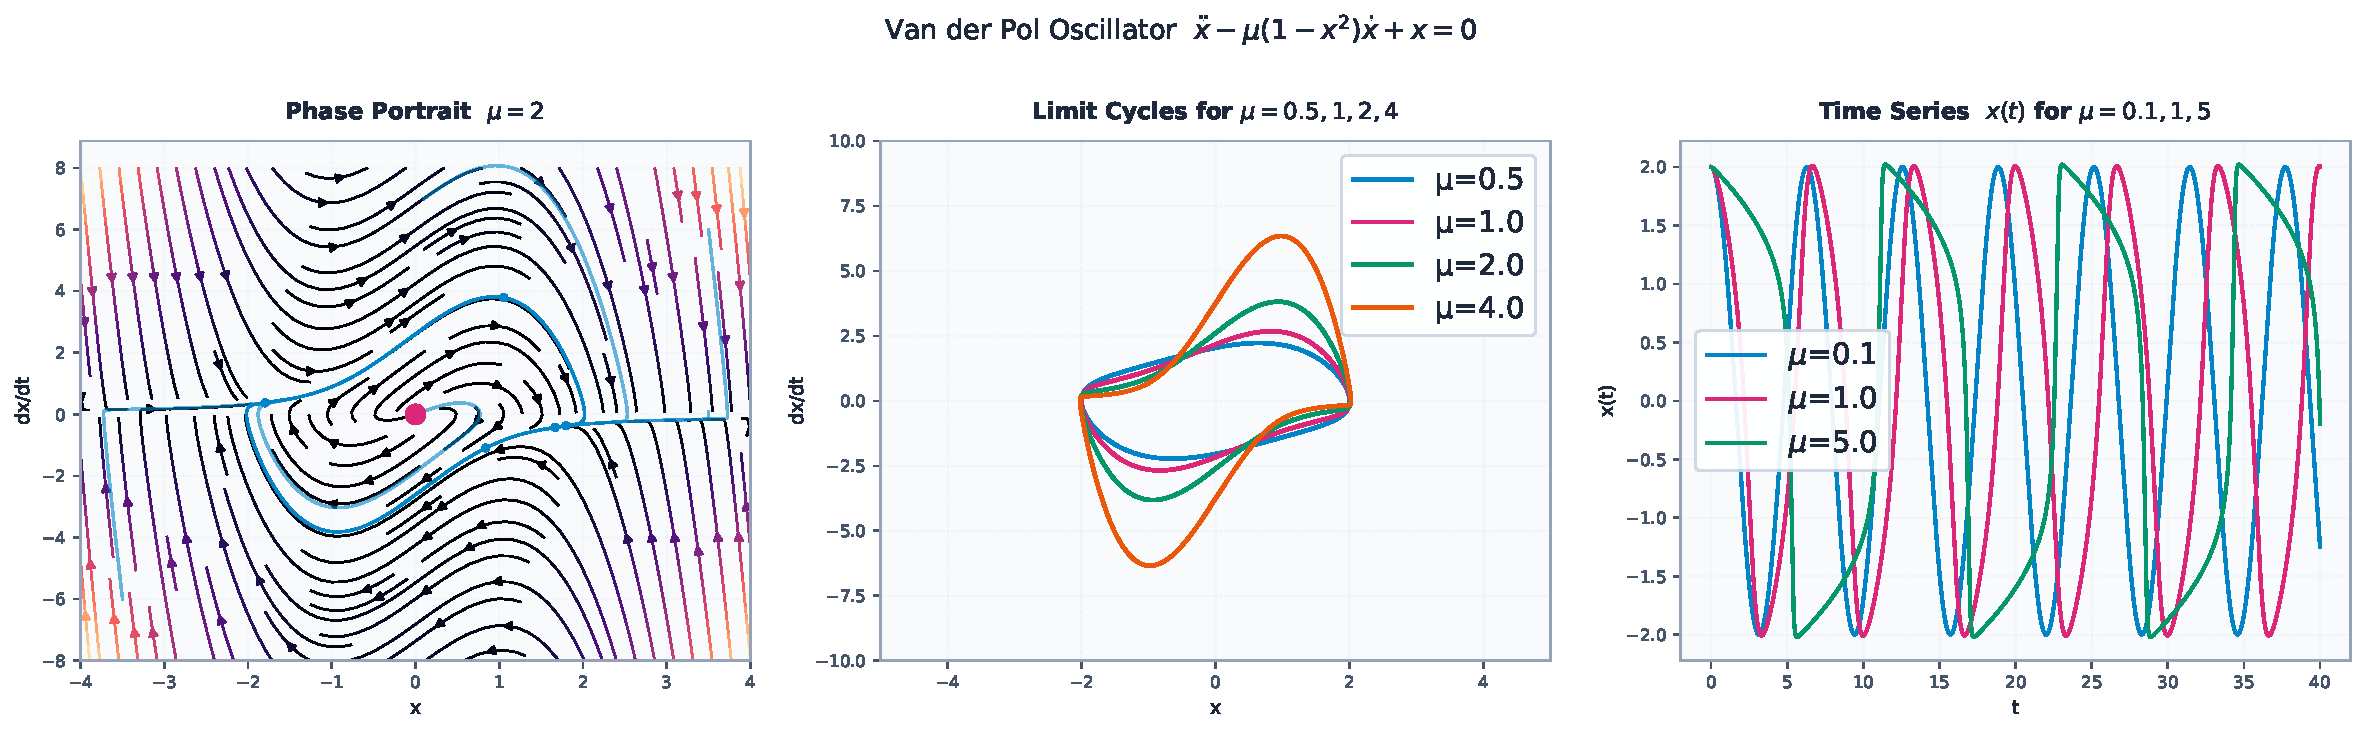
\includegraphics[width=0.8\linewidth, trim={0 0cm 0cm 0cm},clip]{figures/vanderpol_limitcycle.pdf}
\end{center}

\footnotesize

    {\color{mathGray}

    Van der Pol oscillator. \textbf{Left:} Phase portrait ($\mu=2$), all trajectories are attracted to the limit cycle (closed curve), whether starting inside (small initial conditions) or outside (large initial conditions). The unstable fixed point at the origin repels all trajectories. \textbf{Center:} Limit cycles for $\mu=0.5,1,2,4$ , larger $\mu$ produces more relaxation-oscillation character (nearly rectangular shape), with faster transitions. \textbf{Right:} Time series $x(t)$, small $\mu$ gives nearly sinusoidal oscillation; large $\mu$ gives relaxation oscillations with slow-fast dynamics.

    }

    
\end{frame}

\begin{frame}{Bifurcation}


        A bifurcation occurs when the qualitative behaviour of a dynamical system changes as a parameter varies. At a bifurcation value, the structural stability of the system breaks down,  fixed points are created/destroyed, stability changes, or periodic orbits appear.

        \vspace{5pt}


    \begin{tcolorbox}[
    enhanced,
    rounded corners,
    % Set the base thickness for all sides
    boxrule=0.5pt, 
    % Specifically override the left side
    bottomrule=2mm, 
    rightrule = 2mm,
    % Colors
    colframe=white!80!red,
    colback=WarmWhite,
    % Ensure no title space is reserved
    notitle,
    % Optional: Add some padding so text doesn't touch the thick edge
    left=1mm ]

    We consider a parametrized system $\xdot = f(x, r)$. $r = r_c$ is a bifurcation point if the phase portrait for $r < r_c$ is not topologically equivalent to the phase portrait for $r > r_c$.


    

    \end{tcolorbox}


    
\end{frame}

\begin{frame}{Bifurcation in 1-D}

    \resizebox{0.9\textwidth}{!}
{
\begin{tabular}{|p{4.0cm}|p{3.0cm}|p{3.0cm}|p{5.0cm}|p{4.0cm}|}
\hline
\textbf{Bifurcation} & \textbf{Normal Form} & \textbf{Description} & \textbf{Signature} \\
\hline
\textbf{Saddle-Node} & $\dot{x} = r + x^2$ & Two FPs collide and annihilate at $r=0$ & One new stable, one unstable FP created \\
\hline
\textbf{Transcritical} & $\dot{x} = rx - x^2$ & Two FPs exchange stability at $r=0$ & Always two FPs; stability swaps \\
\hline
\textbf{Supercritical Pitchfork} & $\dot{x} = rx - x^3$ & Stable FP loses stability; two new stable FPs appear & Symmetry breaking; soft onset \\
\hline
\textbf{Subcritical Pitchfork} & $\dot{x} = rx + x^3$ & Unstable FP gains stability; two unstable FPs disappear & Hysteresis; hard transition \\
\hline
\end{tabular}
}

    
\end{frame}


\begin{frame}{Hopf Bifurcation: Bifurcation in 2D}

        \begin{tcolorbox}[
    enhanced,
    rounded corners,
    % Set the base thickness for all sides
    boxrule=0.5pt, 
    % Specifically override the left side
    bottomrule=2mm, 
    rightrule = 2mm,
    % Colors
    colframe=white!80!blue,
    colback=WarmWhite,
    % Ensure no title space is reserved
    notitle,
    % Optional: Add some padding so text doesn't touch the thick edge
    left=1mm ]

    Consider $\xdot = f(x, \mu)$ have a fixed point at $x^* = 0$ with eigenvalues $\alpha(\mu ) \pm i \beta (\mu)$. If at $\mu = 0$, (i)$\alpha(0) = 0$, $\beta(0) \neq 0$, (ii) $\frac{d\alpha}{d\mu}|_0 \neq 0$, then as $\mu = 0$, a \textbf{limit cycle bifurcates} from the fixed point. The bifurcation is \textbf{supercritical} (stable cycle) or \textbf{subcritical} (unstable cycle) depending on the sign of a computable coefficient $\sigma$.

        \end{tcolorbox}

    
\end{frame}

\begin{frame}{Bifurcation Diagram}

\footnotesize

        \begin{center}
            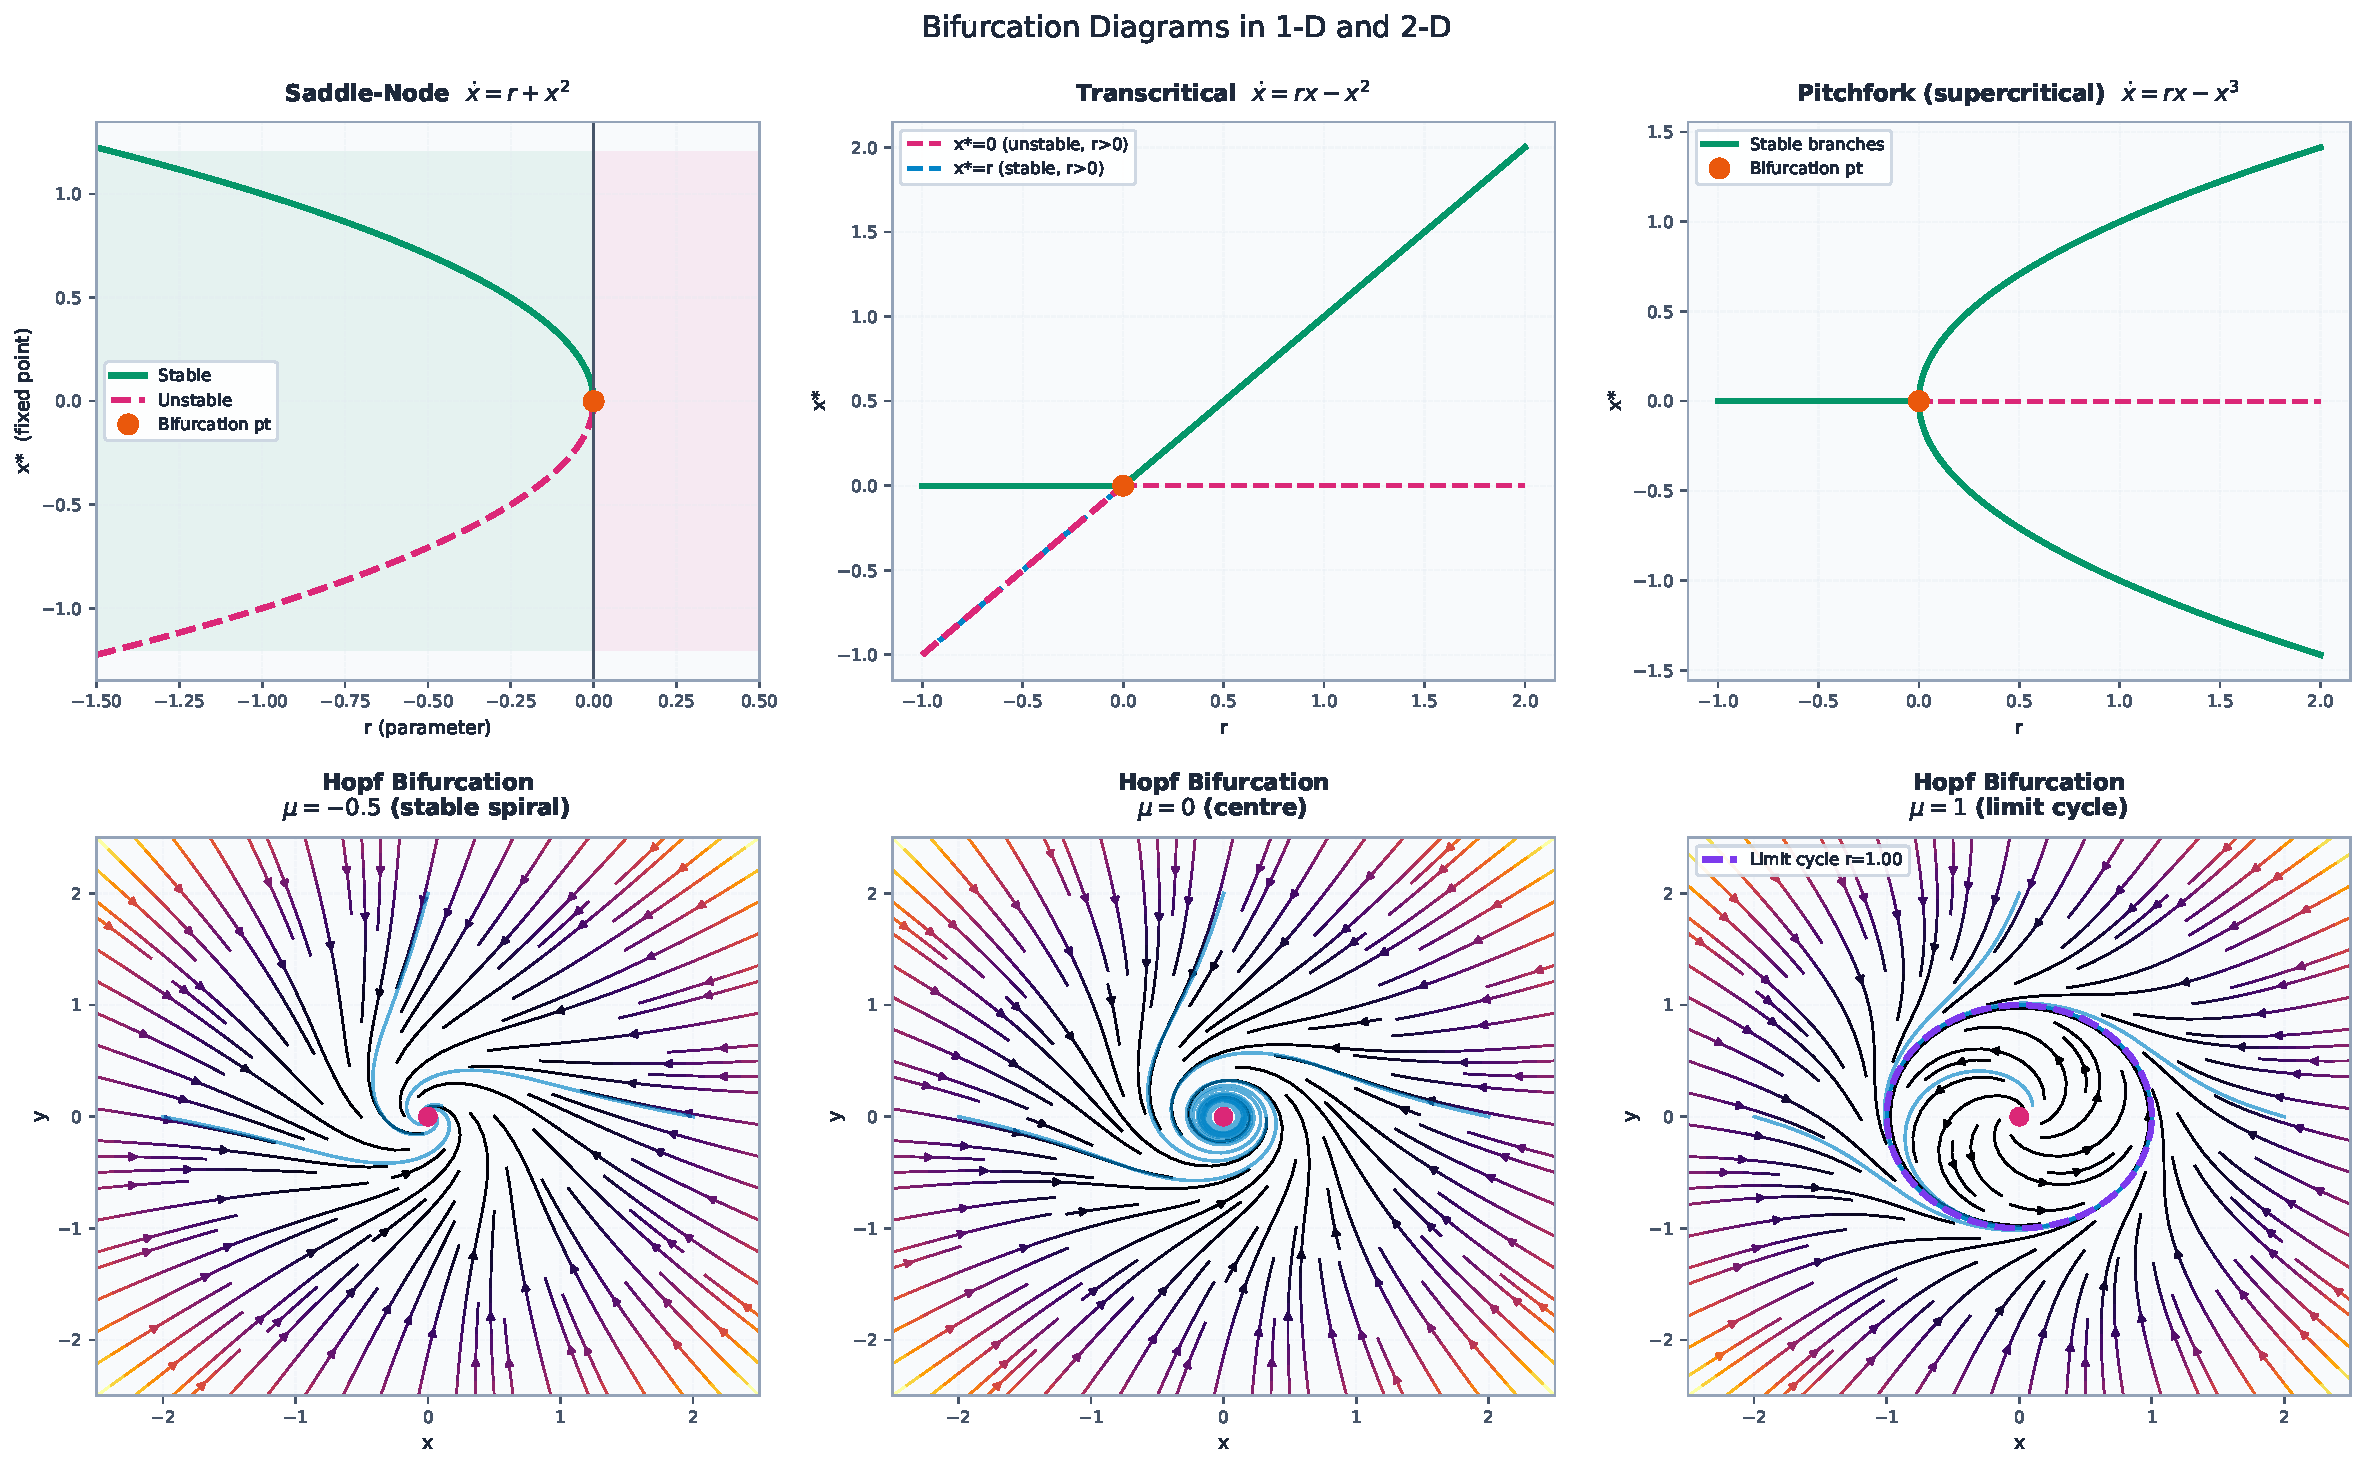
\includegraphics[width=0.6\linewidth, trim={0 0cm 0cm 0cm},clip]{figures/bifurcation.pdf}
\end{center}

\tiny

    {\color{mathGray}

    Bifurcation diagrams. Top row: Three classic 1-D bifurcations, Saddle-Node (two FPs annihilate at $r=0$), Transcritical (stability exchange at $r=0$), Supercritical Pitchfork (symmetry breaking with two new stable branches). Solid lines = stable fixed points; dashed = unstable. Orange star = bifurcation point. Bottom row: Hopf bifurcation in 2-D. At $\mu=-0.5$ (left), the fixed point is a stable spiral. At $\mu=0$ (centre), the fixed point is a centre. At $\mu=1$ (right), the fixed point becomes an unstable spiral and a stable limit cycle (dashed purple circle, radius $\sqrt{\mu}$) appears via Hopf bifurcation.
    }


    
\end{frame}

\begin{frame}{Lyapunov Stability}

        \scriptsize

    A fixed point $x^*$ is Lyapunov stable if $\forall \varepsilon > 0,~~ \exists \delta > 0$ such that $ || x - x^* || < \delta \Rightarrow || \varphi_t(x_0) - x^* || < \varepsilon$ for all $t \geq0 $. 

    \begin{itemize}
        \item A fixed point $x^*$ is asymptotically stable if additionally $\varphi_t(x_0) \to x^*$ as $t \to \infty$. \textbf{A system returns to equlibrium even after being perturbed.} 
        \item  A fixed point $x^*$ is unstable if it is not Lyapunov stable.
        \item  A fixed point $x^*$ is globally asymptotic stable if asymptotically stable with basin of attraction = entire state space.
    \end{itemize}

    \begin{tcolorbox}[title = Lyapunov's Direct Method]
        
        Let $V: U \to\Rbb$ be a smooth function in a neighborhood of $x^* = 0$ with $V(0) = 0$, $V(x) > 0$ for $x \neq 0$ , i.e. positive definition then

        \begin{itemize}
            \item If $\dot{V}(x) = \nabla V \cdot f(x) \leq 0$ on $U /\ \{ 0 \}$ means origin is Lyapunov stable.
            \item If $\dot{V}(x) < 0$ on  $U /\ \{ 0 \}$ means origin is asymptotically stable.
            \item If $\dot{V}(x) > 0$ on  $U /\ \{ 0 \}$ means origin is unstable.
        \end{itemize}

        Here $V$ is called a Lyapunov function.

   

                \begin{tcolorbox}[
                enhanced,
                rounded corners,
                % Set the base thickness for all sides
                boxrule=0.5pt, 
                % Specifically override the left side
                bottomrule=2mm, 
                rightrule = 2mm,
                % Colors
                colframe=white!80!blue,
                colback=WarmWhite,
                % Ensure no title space is reserved
                notitle,
                % Optional: Add some padding so text doesn't touch the thick edge
                left=1mm ]

                $$
                \dot{V} = \frac{dV}{dt} = \nabla V(x) \cdot f(x) = \sum_i \pdv{V}{x_i} f_i(x)
                $$
                \end{tcolorbox}
    \end{tcolorbox}    
\end{frame}

\begin{frame}
    

    \begin{center}
        

\begin{tcolorbox}[
enhanced,
rounded corners,
% Set the base thickness for all sides
boxrule=0.5pt, 
% Specifically override the left side
bottomrule=2mm, 
rightrule = 2mm,
% Colors
colframe=white!80!Green,
colback=WarmWhite,
% Ensure no title space is reserved
notitle,
% Optional: Add some padding so text doesn't touch the thick edge
left=1mm ]

Flow in ODE can be used in engineering and science in applications such as population dynamics, optimal control, fluid mechanics, gradient-based methods, quantum mechanics, etc. Flow map provides a qualitative analysis of a system: fixed points are steady states, and limit cycles are oscillations.

\end{tcolorbox}

    \end{center}

\end{frame}


\section{Stochastic Differential Equation}

\begin{frame}
    \sectionpage
\end{frame}


\begin{frame}{Perturbation in the Experimentally Measured States}

    \footnotesize

\begin{columns}
    \column{0.5\linewidth}
    \begin{tcolorbox}[enhanced, colback=red!5, colframe=red!60!black, boxrule=0.5pt, rightrule = 2mm, leftrule = 0mm, toprule=0mm, bottomrule=0mm,  fonttitle=\bfseries]
    The experimentally measured trajectories of systems modeled by (ODE) do not in fact behave as predicted: the observed state seems to more or less follow the trajectory predicted by (ODE),
    but is apparently subject also to random perturbations.
    
    \vspace{10pt}

    ~~~~ \hfill \indent \textit{\color{Green!70!Yellow}An Introduction to  Stochastic Differential Equations,-- Lawrence C. Evans}
    \end{tcolorbox}
    \column{0.5\linewidth}
    \begin{center}
    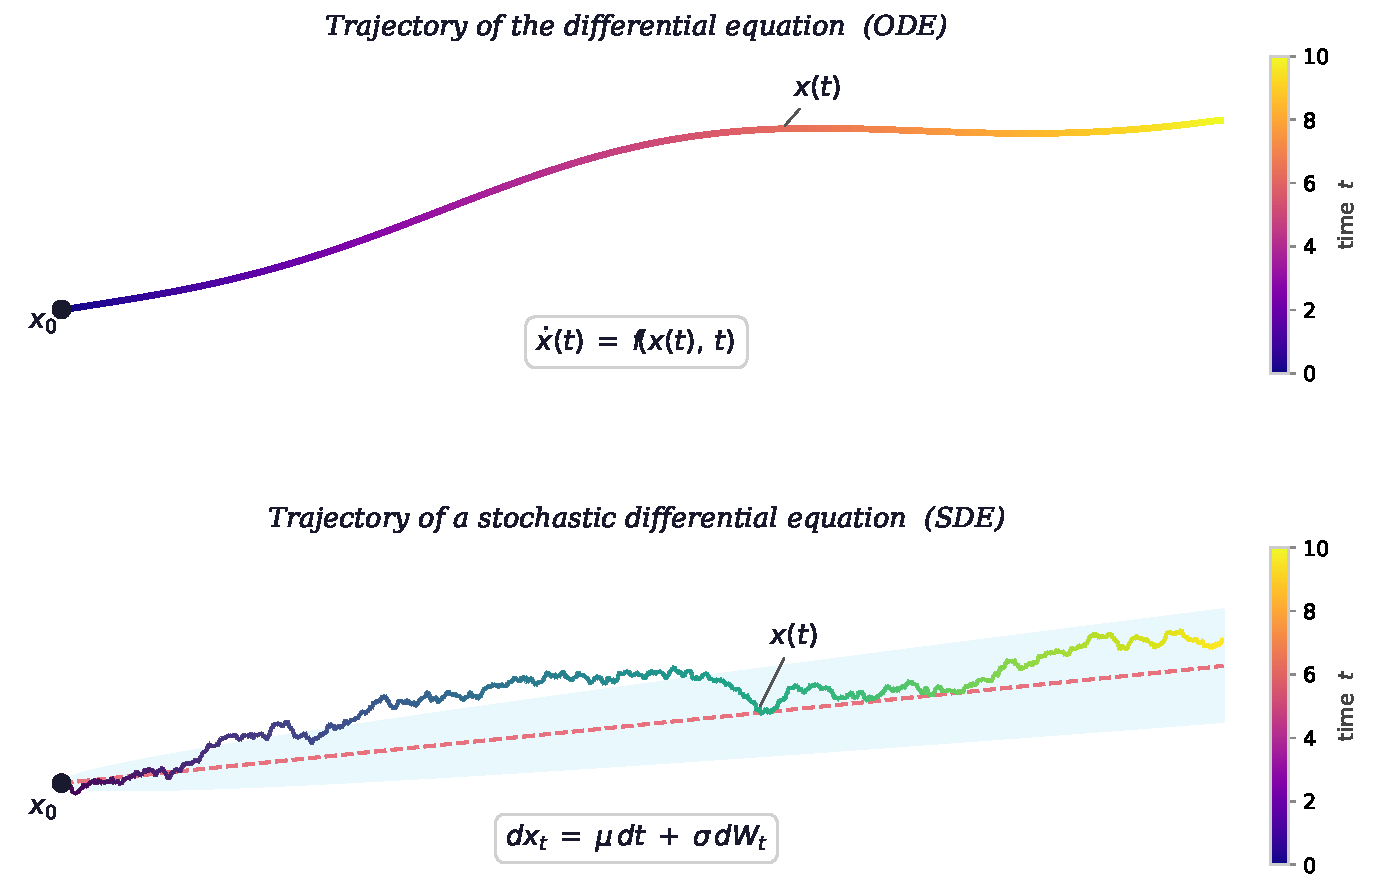
\includegraphics[width=1.0\linewidth]{figures/ode_sde_comparison.pdf}
    \end{center}
    
\end{columns}        
\end{frame}

\begin{frame}{Stochastic Differentials}

    \footnotesize
    
    \begin{align*}
        \frac{d\Xbf(t)}{dt} & = \bbf(\Xbf(t)) + \Bbf(\Xbf(t))\frac{d\Wbf(t)}{dt}\\
        \Rightarrow d\Xbf(t) & = \bbf(\Xbf(t))dt + \Bbf(\Xbf(t))d\Wbf(t)\\
        \Xbf(0) & = x_0
    \end{align*}

    \vspace{3pt}
    Capital bold face to denote multivariate random variable.
    \vspace{3pt}

    \begin{itemize}
        \item $d\Xbf$ and $\Bbf d\Wbf$ are stochastic differentials.
        \item The expression above is calld stochastic differential equation (SDE).
        \item $\Xbf()$ solves SDE provided
        \begin{align*}
            \Xbf(t) = x_0 + \int_0^t \bbf (\Xbf (s))ds + \int_0^t \Bbf(\Xbf(s))d\Wbf \quad \forall t > 0
        \end{align*}

        \item $\Wbf()$ is called Brownian motion or Weiner process. $\xi$ symbol is also used sometimes.
        \item $\int_0^t \cdots d\Wbf$ is stochastic integral.
        \item $x_0 \in \Rbb^n$
        \item $\bbf: \Rbb^n \to \Rbb^n$
        \item $\Bbf: \Rbb^n \to \Mbb^{n\times m}$, = space of $n\times m$ matrices.
    \end{itemize}

\end{frame}

\begin{frame}{Stochastic Differentials}

    \begin{tcolorbox}[enhanced, colback=red!5, colframe=red!60!black, boxrule=0.5pt, leftrule = 2mm, rightrule = 0mm, toprule=0mm, bottomrule=0mm,  fonttitle=\bfseries]
    Question still remains about 
    \begin{itemize}
        \item \textit{Does SDE truly model the physical situation?}
        \item What is the characteristics of $W\bf$?
    \end{itemize}
    
    \end{tcolorbox}


\end{frame}

\begin{frame}{Chain Rule Revisited for Normal Calculus}

    In normal calculus, functions are smooth and well-behaved. They have finite variation. Hence, if you wanna draw the trajectory, you only need finite amount of ink. As the variation is finite, to prove the Chain rule, which computes the dynamics of $f(g(t))$, you only need to take a Taylor expansion of $f(t)$ to the first order. All the higher order terms will tend to zero.

    \begin{columns}
        
    
        \column{0.5\linewidth}
        Using Taylor series, we expand $f(g(t) + dg)$:

            \begin{itemize}
        \item $f'(g)dg$, \textit{keep it}
        \item $\frac{1}{2} f''(g) (dg)^2$ $\to 0$ , $(dt^2 \approx 0)$, \textit{discard}
        \item $\frac{1}{3!}f'''(g)(dg)^3 + \cdots$  $\to 0$, \textit{discard}
    \end{itemize}
    
    For smooth functions, higher-order terms vanish.

    \column{0.5\linewidth}

    \resizebox{0.9\linewidth}{!}{
        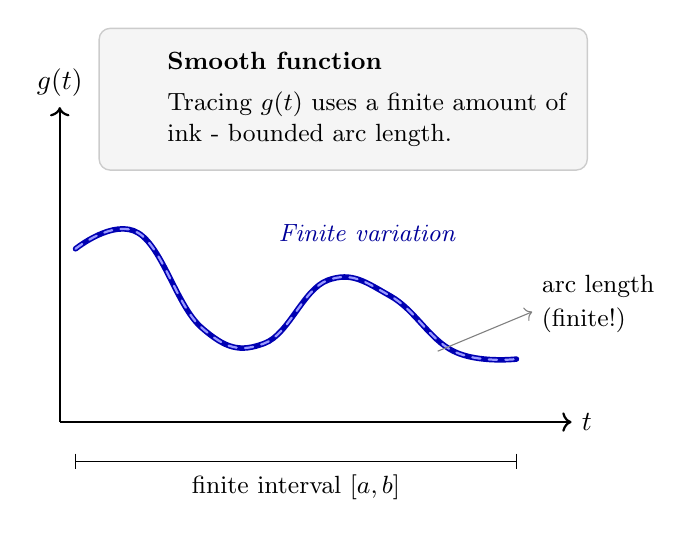
\begin{tikzpicture}[scale=1]
            % Axes
            \draw[->, thick] (0,0) -- (6.5,0) node[right] {$t$};
            \draw[->, thick] (0,0) -- (0,4) node[above] {$g(t)$};

            % Smooth curve
            \draw[blue!70!black, line width=2pt, line cap=round]
                plot[smooth, tension=0.7] coordinates {
                (0.2,2.2) (1.0,2.4) (1.8,1.2) (2.6,1.0)
                (3.4,1.8) (4.2,1.6) (5.0,0.9) (5.8,0.8)
                };

            % Dashed overlay (pencil lead visualisation)
            \draw[blue!40, line width=0.8pt, dashed, line cap=round]
                plot[smooth, tension=0.7] coordinates {
                (0.2,2.2) (1.0,2.4) (1.8,1.2) (2.6,1.0)
                (3.4,1.8) (4.2,1.6) (5.0,0.9) (5.8,0.8)
                };

            % Bracket below
            \draw (0.2,-0.5) -- (5.8,-0.5);
            \draw (0.2,-0.4) -- (0.2,-0.6);
            \draw (5.8,-0.4) -- (5.8,-0.6);
            \node[below] at (3.0,-0.55) {\small finite interval $[a,b]$};

            % Annotation
            \draw[->, gray] (4.8,0.9) -- (6.0,1.4);
            \node[right, align=left] at (6.0,1.5)
                {\small arc length\\\small (finite!)};

            % Caption box
            \draw[rounded corners=4pt, fill=gray!8, draw=gray!40, line width=0.5pt]
                (0.5,3.2) rectangle (6.7,5.0);
            \node[align=left, font=\small] at (3.9, 4.1) {
                \textbf{Smooth function}\\[4pt]
                Tracing $g(t)$ uses a finite amount of\\
                ink - bounded arc length.
            };
            \node[font=\small\itshape, blue!60!black] at (3.9,2.4)
                {Finite variation};
            \end{tikzpicture}
    }


    \end{columns}
\end{frame}

\begin{frame}{Chain Rule When Considering Brownian Motion}

    Brownian motion is so irregular that it has infinite variation. We need infinite amount of ink to draw it.
    
    For that, we have $dW \approx (dt)^{1/2}$.

    \begin{columns}
        \column{0.5\linewidth}
        Taylor expansion of $f(X(t) + dX)$:

        \begin{itemize}
            \item $f'(X)dX$, \textit{keep it}
            \item $\frac{1}{2}f''(X)(dX)^2$ ,  \textit{keep it} $(dW^2 = dt)$
            \item $(dX)^3 + \cdots  \to 0$, \textit{discard}.
        \end{itemize}
        Hence, $df = f'dX + \frac{1}{2}f''(dX)^2$. There is an extra correction term. That's \textbf{Ito's Chain Rule}.

        \column{0.5\linewidth}
    
        \resizebox{1.0\linewidth}{!}{
        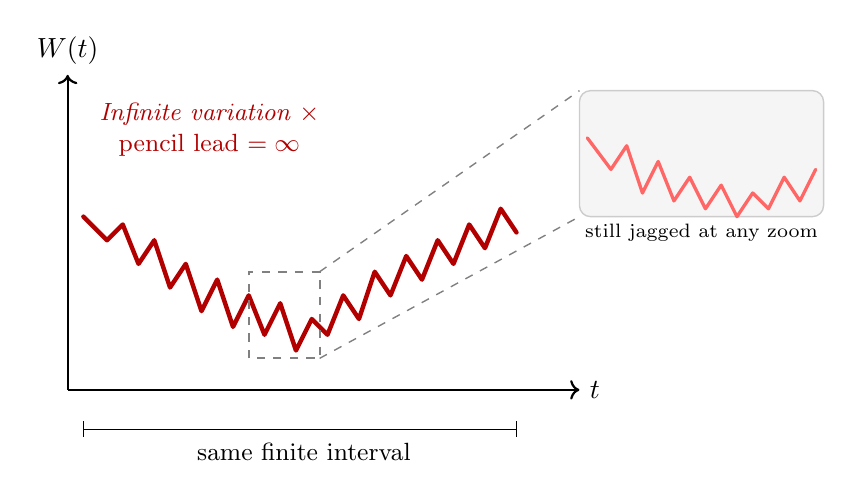
\begin{tikzpicture}[scale=1]
            % Axes
            \draw[->, thick] (0,0) -- (6.5,0) node[right] {$t$};
            \draw[->, thick] (0,0) -- (0,4) node[above] {$W(t)$};

            % Jagged Brownian path
            \draw[red!70!black, line width=1.6pt, line join=round, line cap=round]
                (0.2,2.2) -- (0.5,1.9) -- (0.7,2.1) -- (0.9,1.6)
                -- (1.1,1.9) -- (1.3,1.3) -- (1.5,1.6) -- (1.7,1.0)
                -- (1.9,1.4) -- (2.1,0.8) -- (2.3,1.2) -- (2.5,0.7)
                -- (2.7,1.1) -- (2.9,0.5) -- (3.1,0.9) -- (3.3,0.7)
                -- (3.5,1.2) -- (3.7,0.9) -- (3.9,1.5) -- (4.1,1.2)
                -- (4.3,1.7) -- (4.5,1.4) -- (4.7,1.9) -- (4.9,1.6)
                -- (5.1,2.1) -- (5.3,1.8) -- (5.5,2.3) -- (5.7,2.0);

            % Dashed zoom box on a segment
            \draw[gray, dashed, line width=0.7pt]
                (2.3,0.4) rectangle (3.2,1.5);

            % Leader lines to zoom inset
            \draw[gray, dashed, line width=0.5pt] (3.2,1.5) -- (6.5,3.8);
            \draw[gray, dashed, line width=0.5pt] (3.2,0.4) -- (6.5,2.2);

            % Zoom inset box
            \draw[rounded corners=4pt, fill=gray!8, draw=gray!40, line width=0.5pt]
                (6.5,2.2) rectangle (9.6,3.8);
            % Mini jagged path inside zoom
            \draw[red!60, line width=1.2pt, line join=round, line cap=round]
                (6.6,3.2) -- (6.9,2.8) -- (7.1,3.1) -- (7.3,2.5)
                -- (7.5,2.9) -- (7.7,2.4) -- (7.9,2.7) -- (8.1,2.3)
                -- (8.3,2.6) -- (8.5,2.2) -- (8.7,2.5) -- (8.9,2.3)
                -- (9.1,2.7) -- (9.3,2.4) -- (9.5,2.8);
            \node[font=\scriptsize, align=center] at (8.05,2.0)
                {still jagged at any zoom};

            % Bracket below
            \draw (0.2,-0.5) -- (5.7,-0.5);
            \draw (0.2,-0.4) -- (0.2,-0.6);
            \draw (5.7,-0.4) -- (5.7,-0.6);
            \node[below] at (3.0,-0.55) {\small same finite interval};

            % Infinite variation label
            \node[font=\small\itshape, red!70!black] at (1.8,3.5)
                {Infinite variation $\times$};
            \node[font=\small, red!70!black] at (1.8,3.1)
                {pencil lead $= \infty$};
            \end{tikzpicture}
        }

    \end{columns}
    
\end{frame}


\begin{frame}{Ito's Chain Rule (Ito's Lemma)}

    \footnotesize

    Assume $n = m  = 1$, and a smooth function $u(x): \Rbb \to \Rbb$, then $dX = b(X) dt + dW$

    \vspace{5pt}
    
    We can ask what stochastic differential equation does $Y(t) := u(X(t))$ solve?
    
    \vspace{3pt}

    From normal calculus, $dY = u'dX = u'bdt + u'dW$ where $' = \frac{d}{dx}$.

    
    \vspace{10pt}

    \textbf{But that's not the cae when $W$ is a Brownian Motion. Above calculation will be wrong.}

    So in Taylor series expansion, 

    \begin{align*}
        dY & = u'dX + \frac{1}{2}u'' (dX)^2\\
            & = u'(bdt + dW) + \frac{1}{2}u''(bdt + dW)^2 + \cdots\\
            & = \bigg ( u'b  + \frac{1}{2}u''\bigg) dt + u'dW + \{ \text{ terms of order } (dt)^{3/2} \text{ and higher } \}
    \end{align*}
    We used $(dW)^2 = dt$. Compared to ordinary calculus, we see an extra term $\frac{1}{2}u''dt$.


    
\end{frame}

\begin{frame}{Example}

    \scriptsize 

    Find the solution to SDE:

    \begin{align*}
        dY & = YdW \\
        Y(0) = 1
    \end{align*}

    We guess the solution has the form $Y(t) = e^{f(t, W(t))}$ for some function $f$ and use Ito's Lemma to find $f$.

    \vspace{5pt}

    \pause 

    \textbf{Step 1:} Make an ansatz (fancy name for making a guess): $Y(t) = e^{aW(t) + bt}$ for some constant $a$, and $b$. We define $u(x, t) = e^{ax + bt}$ for convenience. Thus, $Y() = u(W(t), t)$.

    \vspace{5pt}

    \pause 

    \textbf{Step 2:} For a smooth $u(x, t)$, Ito's Lemma gives 

    \begin{align*}
        du  = \pdv{u}{t}dt + \pdv{u}{x}dW+ \frac{1}{2}\pdv[2]{u}{x} dt
    \end{align*}

    Compute the partials of $u = e^{ax + bt}$: 

    \begin{align*}
        \pdv{u}{t} = be^{ax + bt}, \quad \pdv{u}{x} = a e^{ax + bt}, \quad \pdv[2]{u}{x} = a^2 e^{ax + bt}
    \end{align*}
    Then,  $dY = bYdt + a YdW + \frac{1}{2}a^2 Y dt = \bigg( b + \frac{a^2}{2} \bigg) Y dt + aY dW$.

    
\end{frame}

\begin{frame}{Example continues ...}

    \textbf{Match coefficients}

    We need $dY = Y dW$ (that's what the original question is). Comparing coefficients:

    \begin{align*}
        \bigg( b + \frac{a^2}{2} \bigg) Y dt + aY dW =  0\cdot Y dt + 1\cdot Y dW
    \end{align*}
    
    $ a= 1$, $ b + \frac{a^2}{2} = 0 \Rightarrow b  = -\frac{1}{2}$.
    
    \vspace{5pt}

    \pause 

    Putting into our ansatz:
    \begin{align*}
        Y(t) = e^{W(t) - \frac{1}{2}t}. 
    \end{align*}
    which also satisies $Y(0) = e^{W(0) - 0} = e^0 = 1$. We have $W(0) = 0$ by the definition of Brownian motion.
\end{frame}

\begin{frame}{Brownian Motion}

    \textbf{Brownian Motion} is a fundamental stochastic process that came out of studying actual diffusion process in the nature.

    \vspace{10pt}

        \begin{tcolorbox}[enhanced, colback=red!5, colframe=red!60!black, boxrule=0.5pt, rightrule = 2mm, leftrule = 0mm, toprule=0mm, bottomrule=0mm,  fonttitle=\bfseries]
            A Brownian motion $W = (W_t)_{0 \leq t \leq 1}$ is a stochastic process such that $W_0 = 0$, the trajectories $ t \mapsto W_t$ are continuous and holds two condition:
            \begin{enumerate}
                \item Normal increment: $W_t - W_s \sim \Ncal(0, (t-s)I_d)$ for all $ 0 \leq s \leq t $, i.e. increments have Gaussain distribution with variance increasing linearly in time ($I_d$ is the identity matrix).
                \item Independent increments: Increments $W_{t_1} - W_{t_0}, \cdots , W_{t_n} - W_{t_{n-1}}$ are independent random variables.
            \end{enumerate}
        \end{tcolorbox}

        \scriptsize

        Brownian motion is called Weiner process. We can simulate Brownian motion with a step size $h$, such that $ t= 0, h, 2h, \cdots $ and $W_0 = 0$ such that $W_{t+1} = W_t + \sqrt{h}\epsilon_t$, $\epsilon_t \sim \Ncal(0, I_d)$.
    
\end{frame}

\begin{frame}{Simulating an ODE}

    Numerically, there is a rich theory and implementation on simulating a numerical ODE. Most simple one is the Euler method.

    $$
    X_{t+h} = X_t + h u_t(X_t), \quad t = 0, h, 2h, \cdots
    $$
    
\end{frame}

\begin{frame}
    A flow model can be described by an ODE as 

    \begin{align*}
        X_0 \sim p_{init} \quad \textbf{random initiliazation}, p_{init}  = \Ncal(0, I_d)\\
        \frac{d}{dt}X_t = u_t^\theta(X_t) \quad \textbf{ODE}
    \end{align*}
    Our goal is made endpoint trajectory $X_{end} \sim p_{data} \Leftrightarrow \psi_{end}^\theta(X_0) \sim p_{data}$
    where $\psi_t^\theta$ describes the flow induced by $u_t^\theta$.

    \begin{itemize}
        \item Here, $u_t^\theta$ would be called \textbf{Neural Network vector field}.
    \end{itemize}
\end{frame}

\begin{frame}{Sampling from a Flow Model with Euler Method}

\begin{algorithm}[H]
    \caption{\textbf{Sampling from a Flow Model with Euler method}}
    \DontPrintSemicolon
    
    \KwRequire{Neural network vector field $u_t^\theta$, number of steps $n$}
    
    Set $t = 0$\;
    Set step size $h = \frac{1}{n}$\;
    Draw a sample $X_0 \sim p_{\text{init}}$\;
    
    \For{$i = 1, \dots, n$}{
        $X_{t+h} = X_t + h u_t^\theta(X_t)$\;
        Update $t \leftarrow t + h$\;
    }
    
    \KwRet $X_1$\;
\end{algorithm}
    
\end{frame}

\begin{frame}{From ODE to SDE}
{\scriptsize \url{https://web.archive.org/web/20260319034510/https://diffusion.csail.mit.edu/2026/docs/lecture_notes.pdf}}

\vspace{5pt}

We can rewrite ODE trajectories as 

\begin{align*}
    & \frac{d}{dt} X_t = u_t(X_t)\\
    \Leftrightarrow & \frac{1}{h} (X_{t+h}  - X_t) = u_t(X_t)  + R_t(h)\\
    \Leftrightarrow & X_{t+h} = X_t + h u_t (X_t) + h R_t(h)
\end{align*}

where $R$ is some function such that $\lim_{h \to 0} R_t(h) = 0$ which is an error term in numerical method.

To make it stochastic, we add one more term:

\begin{align*}
    X_{t+h} = X_t + hu_t(X_t) + \sigma_t(W_{t+h} - W_t) + h R_t(h)
\end{align*}

$\sigma_t$ is diffusion coefficient.

    
\end{frame}

\begin{frame}{An Example of an SDE Process}

Let's have a constant diffusion coefficient $\sigma_t = \sigma \geq 0 $ and  a constant linear drift $u_t(x ) = -\theta x$ for $\theta > 0$ which gives us

\begin{align*}
    dX_t = - \theta X_t dt + \sigma dW_t
\end{align*}

A solution to this SDE is called \textbf{ Ornstein - Uhlenbeck Process}.
    
\end{frame}

\begin{frame}{Simulating an SDE}

    The simplest method is \textbf{Euler - Maruyama} method.

    \vspace{5pt}

    Initialize $X_0 = x_0$ and update iteratively as 

    $$
    X_{t+h} = X_t + h u_t(X_t) + \sqrt{h}\sigma_t \epsilon_t, \quad \epsilon_t \sim \Ncal(0, I_d)
    $$
    
\end{frame}

\begin{frame}{Diffusion Model with SDE}

    A diffusion model is thus given by 

    \begin{align*}
        & X_0 \sim p_{init}\\
        & dX_t = u_t^\theta (X_t)dt + \sigma_t dW_t
    \end{align*}

    \scriptsize

    \begin{algorithm}[H]
    \caption{\textbf{Sampling from a Diffusion Model (Euler-Maruyama method)}}
    \DontPrintSemicolon
    
    \textbf{\color{blue}Require:} Neural network $u_t^\theta$, number of steps $n$, diffusion coefficient $\sigma_t$\;
    
    Set $t = 0$\;
    Set step size $h = \frac{1}{n}$\;
    Draw a sample $X_0 \sim p_{\text{init}}$\;
    
    \For{$i = 1, \dots, n$}{
        a sample $\epsilon \sim \mathcal{N}(0, I_d)$\;
        $X_{t+h} = X_t + h u_t^\theta(X_t) + \sigma_t \sqrt{h} \epsilon$\;
        Update $t \leftarrow t + h$\;
    }
    \textbf{\color{blue}return} $X_1$
\end{algorithm}
    
\end{frame}


\begin{frame}{Flow Matching}

    We saw how can be use a neural network to construct flow and diffusion model.

    But

    \Large 
    \vspace{10pt}
    
    \textbf{How to train them !}
    
\end{frame}

\begin{frame}{References}
\footnotesize
    \begin{itemize}
    \item \textbf{Original Paper} on Diffusion Model, Deep Unsupervised Learning using Nonequilibrium Thermodynamics: \url{https://proceedings.mlr.press/v37/sohl-dickstein15.pdf}
    \item \textbf{The Most Influential Paper:} Denoising Diffusion Probabilistic Models \url{https://arxiv.org/pdf/2006.11239}
        \item Deep Learning Notes by Prof. LI Hongsheng: \url{https://dl.ee.cuhk.edu.hk/slides/diffusion.pdf}
        
        \item Diffusion Models: A Comprehensive Survey of Methods and Applications: \url{https://dl.acm.org/doi/full/10.1145/3626235?casa_token=tLriJS0Ll7EAAAAA:G_ue_8JwODm_PGRul_bBdK70QpTLetomFM1ioVMzebrqCaAtiozqPpcs2hV62SMAUIz01-TvweBV}
        \item Understanding Diffusion Models: A Unified Perspective: \url{https://arxiv.org/pdf/2208.11970.pdf}
        \item U-Net: Convolutional Networks for Biomedical Image Segmentation: \url{https://arxiv.org/pdf/1505.04597.pdf}
        \item ConvNext: A ConvNet for the 2020s: \url{https://arxiv.org/pdf/2201.03545.pdf}
        \item ACC-UNet: A Completely Convolutional UNet model for the 2020s: \url{https://arxiv.org/pdf/2308.13680.pdf}
        \item Latent Diffusion Paper: \url{https://arxiv.org/pdf/2112.10752.pdf}
    \end{itemize}
\end{frame}
    
\begin{frame}{References}
    \begin{itemize}
        \item Stable Diffusion Github Repo: \url{https://github.com/CompVis/stable-diffusion?tab=readme-ov-file}
        \item Diffusion Models Beat GANs on Image Synthesis (Guided Diffusion): \url{https://arxiv.org/pdf/2105.05233.pdf}
        \item Guided Diffusion Github Repo: \url{https://github.com/openai/guided-diffusion}
    \end{itemize}
\end{frame}

\begin{frame}{Let's do some coding}
    \begin{center}
        \LARGE
        \url{https://github.com/rahulbhadani/CPE487587_SP26/blob/master/Code/Chapter_08_DiffusionModel.ipynb}
    \end{center}
\end{frame}

%------------------------------------------------
\begin{frame}
    \Huge{\centerline{\color{MediumBlue}\textbf{The End}}}
\end{frame}
    
\end{document}